\documentclass[semifinal,survey]{cpecmu}
%% หมายเหตุ: ตัวเลือก semifinal จะแสดงแถบดำตรงบรรทัดที่ล้นขอบ (overfull hbox)
%% เมื่อพร้อมส่งฉบับจริง ให้เปลี่ยนเป็น \documentclass[final]{cpecmu}

%% TODO: ใส่เลขที่โครงงานที่ภาควิชากำหนดให้ (ตอนนี้ยังไม่ทราบ)
\projectNo{S007-1}
%% ปีการศึกษา (ค.ศ.) ระบบจะแปลงเป็น พ.ศ. ให้อัตโนมัติ: 2026 -> 2569
\acadyear{2026}

\titleTH{การใช้โมเดลภาษาขนาดใหญ่วิเคราะห์บันทึกเหตุการณ์จากระบบบริหารจัดการข้อมูลและเหตุการณ์ด้านความปลอดภัย}
\titleEN{Using LLM to Analyze SIEM Logs}

%% TODO: ตรวจสอบคำนำหน้าชื่อและการสะกดชื่อภาษาอังกฤษให้ตรงกับทะเบียน
\author{นายธนกร เสาคำ}{Thanakon Saokham}{660610761}
\author{นางสาวนพรดา กฤษวัฒนานนท์}{Nopparada Kritwattananont}{660610766}
\author{นายบูรณิน บุณโยประการ}{Buranin Boonyoprakan}{660610770}

%% อาจารย์ที่ปรึกษาและกรรมการ (ชื่อดึงมาจาก cpecmu-faculty.sty)
\cpeadvisor{yuthapong}   % ผศ.ดร.ยุทธพงษ์ สมจิต
\cpecommittee{trasapong} % รศ.ดร.ตรัสพงศ์ ไทยอุปถัมภ์
\cpecommittee{sasin}     % ผศ.ดร.ศศิน จันทร์พวงทอง
\cpecommittee{karn}      % ผศ.ดร.กานต์ ปทานุคม

%% Packages
\usepackage[final]{graphicx} % for including graphics
\graphicspath{{figures/}}
\usepackage{amsmath}
\usepackage{array}
\usepackage[section]{placeins} % ไม่ให้รูป/ตารางลอยข้ามหัวข้อ
\usepackage{needspace} % กันหัวข้อกับเนื้อหาแยกหน้า
\usepackage{capt-of}   % ใส่ caption ให้รูปที่ไม่ลอย (\captionof)
\setcounter{secnumdepth}{3} % ให้หัวข้อระดับ x.x.x.x มีเลข (ใช้ในบทที่ 3)
\setcounter{tocdepth}{3}
\newcolumntype{L}[1]{>{\raggedright\arraybackslash}p{#1}}
\usepackage{tikz}
\usetikzlibrary{arrows.meta,positioning,fit,backgrounds}

%% Add bookmarks and hyperlinks in the document.
\PassOptionsToPackage{hyphens}{url}
\usepackage[colorlinks=true,allcolors=Blue4,citecolor=red,linktoc=all]{hyperref}
\def\UrlLeft#1\UrlRight{$#1$}

\usepackage{afterpage}
\usepackage{pdflscape}

%% ช่วยลดปัญหาบรรทัดล้นขอบ (overfull hbox) จากการตัดคำภาษาไทย
\setlength{\emergencystretch}{3em}

%% ไม่ตัดคำภาษาอังกฤษด้วยขีด (-) ตอนท้ายบรรทัด เช่น Inves-tigation
\hyphenpenalty=10000

\bibliographystyle{unsrt} % เรียงเลขอ้างอิงตามลำดับที่ปรากฏในเนื้อหา

\begin{document}
\maketitle
\makesignature

\ifproject
\begin{abstractTH}
โครงงานนี้ประเมินแนวทางการสร้าง Investigation Context จาก Security Logs ในระบบ SIEM
ก่อนส่งให้โมเดลภาษาขนาดใหญ่ (LLM) วิเคราะห์ เพื่อแก้ปัญหาข้อมูลจำนวนมาก, Noise
และต้นทุน Token ที่สูงจากการใช้ Raw Logs โดยตรง
โครงงานพัฒนา Context Construction Pipeline ที่คัดกรองและจัดรูปแบบเฉพาะข้อมูลที่เกี่ยวข้องกับเหตุการณ์
ร่วมกับการอ้างอิงองค์ความรู้จาก MITRE ATT\&CK เพื่อให้ LLM ขนาดเล็กที่ใช้ทำงานภายในเครื่อง
สามารถระบุเทคนิคการโจมตีได้อย่างแม่นยำ
ผลลัพธ์จะถูกนำเสนอเป็นรายงานการสืบสวน (Investigation Report) ผ่าน Web Dashboard
เพื่อช่วยให้ SOC Analyst ลดเวลาในการสืบสวนเหตุการณ์ และลดต้นทุนในการใช้ LLM
โดยยังคงหลักฐานที่จำเป็นต่อการวิเคราะห์ไว้ครบถ้วน
\end{abstractTH}

\begin{abstract}
This project evaluates approaches for constructing an investigation context from
security logs collected by a Security Information and Event Management (SIEM) system
before they are analyzed by a large language model (LLM).
Feeding raw logs directly to an LLM is problematic because of the large data volume,
the amount of irrelevant information (noise), and the resulting high token cost.
We develop a Context Construction Pipeline that normalizes the logs, selects only the
events related to the alerted incident, and formats them in a compact representation,
combined with knowledge retrieved from the MITRE ATT\&CK framework, so that a small
LLM running locally can accurately identify the attack technique.
The analysis is presented as an investigation report on a web dashboard, helping SOC
analysts reduce investigation time and LLM usage cost while preserving the evidence
required for the analysis.
\end{abstract}

\iffalse
\begin{dedication}
Dedication page is optional.
\end{dedication}
\fi % \iffalse

% \begin{acknowledgments}
% โครงงานนี้สำเร็จลุล่วงได้ด้วยความกรุณาจาก ผศ.ดร.ยุทธพงษ์ สมจิต อาจารย์ที่ปรึกษาโครงงาน
% ที่ได้สละเวลาให้คำปรึกษา ข้อเสนอแนะ และแนวทางในการดำเนินงานตลอดระยะเวลาการทำโครงงาน
% คณะผู้จัดทำขอกราบขอบพระคุณเป็นอย่างสูงมา ณ ที่นี้

% ขอขอบพระคุณคณะกรรมการสอบโครงงาน ได้แก่ รศ.ดร.ตรัสพงศ์ ไทยอุปถัมภ์
% ผศ.ดร.ศศิน จันทร์พวงทอง และ ผศ.ดร.กานต์ ปทานุคม
% ที่ได้ให้คำถามและข้อเสนอแนะอันเป็นประโยชน์ระหว่างการนำเสนอ
% ซึ่งช่วยให้คณะผู้จัดทำปรับปรุงการนิยามปัญหา ขอบเขต และวิธีการทดลองให้ชัดเจนยิ่งขึ้น

% ขอขอบคุณภาควิชาวิศวกรรมคอมพิวเตอร์ คณะวิศวกรรมศาสตร์ มหาวิทยาลัยเชียงใหม่
% ที่ให้ความรู้และสนับสนุนการทำโครงงาน
% รวมถึงผู้พัฒนาชุดข้อมูลสาธารณะ Splunk Attack Data และ OTRF Security-Datasets
% ที่ทำให้การทดลองในโครงงานนี้เป็นไปได้

% \acksign{2026}{10}{22}
% \end{acknowledgments}%
\fi % \ifproject

\contentspage

\ifproject
\figurelistpage

\tablelistpage
\fi % \ifproject


\pagestyle{empty}\cleardoublepage
\normalspacing \setcounter{page}{1} \pagenumbering{arabic} \pagestyle{cpecmu}

\chapter{\ifenglish Introduction\else บทนำ\fi}

\section{\ifenglish Project rationale\else ที่มาของโครงงาน\fi}

ระบบ Security Information and Event Management (SIEM) ทำหน้าที่รวบรวม Security Logs
จากแหล่งข้อมูลจำนวนมากในองค์กร เช่น เครื่องลูกข่าย เซิร์ฟเวอร์ และอุปกรณ์เครือข่าย
แล้วนำมาจัดเก็บ ค้นหา และสร้างการแจ้งเตือน (Alert) เมื่อพบพฤติกรรมที่น่าสงสัย
อย่างไรก็ดี ปริมาณและความหลากหลายของ Logs ทำให้การสืบสวนเหตุการณ์ทำได้ยาก
ตัวอย่างเช่น ชุดข้อมูลจำลองการโจมตีแบบ Account Discovery (T1087.001)
จาก Splunk Attack Data~\cite{splunk-attack-data} มี Windows Sysmon Logs ถึง 11,090 events
ที่เกิดขึ้นภายในเวลาประมาณ 15 นาที (ขนาดไฟล์ XML ประมาณ 16.8 MB)
ซึ่งมีเพียงส่วนน้อยเท่านั้นที่เกี่ยวข้องกับการโจมตีจริง

แม้ Alert จาก SIEM หรือ Endpoint Detection and Response (EDR) จะช่วยชี้ Event หรือกิจกรรมที่ควรตรวจสอบ
แต่การระบุว่าเหตุการณ์ดังกล่าวเป็นการโจมตีหรือไม่ และสอดคล้องกับเทคนิคใดใน MITRE ATT\&CK~\cite{mitre-attack}
ยังต้องอาศัย SOC Analyst ในการรวบรวมและเชื่อมโยง Logs ที่เกี่ยวข้องเข้าด้วยกัน
ซึ่งใช้เวลาและความเชี่ยวชาญสูง

แนวทางหนึ่งที่ได้รับความสนใจคือการใช้โมเดลภาษาขนาดใหญ่ (Large Language Model: LLM) ช่วยวิเคราะห์ Logs
แต่การส่ง Raw Logs ให้ LLM โดยตรงมีปัญหาสำคัญ 2 ประการ ได้แก่
(1) ต้นทุนด้าน Token สูง เนื่องจาก Logs มีขนาดใหญ่และมีโครงสร้างซ้ำซ้อน และ
(2) Logs มี Noise จำนวนมาก (เหตุการณ์ที่ไม่เกี่ยวข้องกับการวิเคราะห์ รวมถึง Field และ Event ที่ไม่จำเป็น)
ซึ่งทำให้ LLM ตีความผิดพลาดได้ง่าย
จากการทดลองเบื้องต้นของคณะผู้จัดทำ เมื่อส่ง Raw Logs ของชุดข้อมูล T1087.001 ที่ดึงจาก Splunk ผ่าน API
ให้ LLM เชิงพาณิชย์หลายตัววิเคราะห์โดยตรง พบว่าบางโมเดลระบุเทคนิคผิด
(เช่น ตอบเป็น T1003 OS Credential Dumping) บางโมเดลสรุปว่าไม่พบการโจมตี
และแม้โมเดลที่ตอบใกล้เคียงที่สุดก็ระบุได้เพียงระดับ Technique (T1087) แต่ไม่ถึงระดับ Sub-technique ที่ถูกต้อง

ด้วยเหตุนี้ โครงงานนี้จึงมุ่งออกแบบและประเมิน \textbf{Context Construction Pipeline}
ที่ทำหน้าที่สร้าง \textbf{Investigation Context} ซึ่งหมายถึงชุดเหตุการณ์และความรู้ที่เกี่ยวข้องกับเหตุการณ์ที่น่าสงสัย
ที่ถูกจัดเตรียมไว้เพื่อให้ LLM ใช้เหตุผลกับเหตุการณ์นั้น
โดย Pipeline จะนำ Alert เป็นจุดเริ่มต้นการสืบสวน แล้วทำการ Normalize, คัดเลือก Event ที่เกี่ยวข้อง (Event Selection)
และแปลงรูปแบบข้อมูล (Representation) ให้กระชับ ก่อนเสริมด้วยองค์ความรู้จาก MITRE ATT\&CK
ผ่าน Retrieval-Augmented Generation (RAG)~\cite{lewis2020rag}
เพื่อให้ LLM ขนาดเล็กที่ทำงานภายในเครื่อง (Local LLM) สามารถระบุเทคนิคการโจมตีได้อย่างแม่นยำ
โดยไม่ต้องส่งข้อมูล Logs ขององค์กรออกไปยังบริการภายนอก

\section{\ifenglish Objectives\else วัตถุประสงค์ของโครงงาน\fi}
\begin{enumerate}
    \item เพื่อออกแบบและพัฒนา Context Construction Pipeline สำหรับสร้าง Investigation Context
          จาก Security Logs ในระบบ SIEM ก่อนส่งให้ LLM วิเคราะห์
    \item เพื่อเปรียบเทียบประสิทธิภาพของวิธีการคัดเลือก Event (Event Selection)
          และรูปแบบการนำเสนอข้อมูล (Representation) แบบต่าง ๆ
    \item เพื่อทดสอบว่า Investigation Context ช่วยเพิ่มความแม่นยำในการระบุเทคนิค MITRE ATT\&CK
          ได้ดีกว่าการใช้ Raw Logs
    \item เพื่อลดปริมาณข้อมูลที่ส่งให้ LLM (ลด Token Cost และลด Noise)
          โดยยังคงหลักฐานที่จำเป็นต่อการวิเคราะห์ไว้ครบถ้วน
    \item เพื่อพัฒนาต้นแบบ Web Dashboard ที่นำเสนอผลการวิเคราะห์เป็นรายงานการสืบสวน (Investigation Report)
          ให้แก่ SOC Analyst
\end{enumerate}

\section{\ifenglish Project scope\else ขอบเขตของโครงงาน\fi}

\subsection{\ifenglish Hardware scope\else ขอบเขตด้านฮาร์ดแวร์\fi}
\begin{enumerate}
    \item ระบบทำงานบนเครื่องคอมพิวเตอร์ส่วนบุคคลหรือเซิร์ฟเวอร์ที่มีหน่วยประมวลผลกราฟิก (GPU)
          เพียงพอสำหรับรัน LLM ขนาดประมาณ 9 พันล้านพารามิเตอร์ (9B) ภายในเครื่อง
    \item ไม่มีการพัฒนาหรือติดตั้งอุปกรณ์ฮาร์ดแวร์เฉพาะทาง เช่น เซนเซอร์หรืออุปกรณ์เครือข่าย
\end{enumerate}

\subsection{\ifenglish Software scope\else ขอบเขตด้านซอฟต์แวร์\fi}
\begin{enumerate}
    \item ใช้ชุดข้อมูลสาธารณะที่มี Ground Truth เพื่อให้ตรวจสอบความแม่นยำได้
          ได้แก่ OTRF Security-Datasets~\cite{otrf-security-datasets} สำหรับออกแบบและวัดผล (Benchmark)
          และ Splunk Attack Data~\cite{splunk-attack-data} สำหรับทดสอบ (Validation)
          โดยนำ Logs ไป Replay เข้า Splunk Enterprise เพื่อจำลองการทำงานของ SIEM จริง
    \item รองรับ Logs ในรูปแบบ Windows Sysmon~\cite{sysmon} และ Linux Auditd~\cite{auditd}
    \item หน่วยของการวิเคราะห์คือ 1 Alert ต่อ 1 กรณีการสืบสวน (Alert-centric)
          โดย Alert ถือเป็น Input ที่ได้รับจาก SIEM/EDR เดิม โครงงานนี้ไม่ได้ทำหน้าที่ตรวจจับภัยคุกคามแทน SIEM/EDR
    \item ใช้ LLM ตัวเดียวตลอดการทดลอง (Qwen3.5 9B ทำงานภายในเครื่องผ่าน Ollama)
          เพื่อให้ Pipeline เป็นตัวแปรเดียวที่เปลี่ยนแปลงในการทดลอง
    \item Ground Truth อยู่ในระดับ Scenario Dataset กล่าวคือ 1 Scenario Dataset มีเทคนิค ATT\&CK
          ที่เป็นเฉลยหนึ่งเทคนิค ซึ่งใช้สำหรับประเมินผลเท่านั้น ไม่ได้นำไปใช้ฝึกสอนโมเดล
    \item ผลลัพธ์ของระบบคือเทคนิค MITRE ATT\&CK ที่ระบุได้ พร้อมหลักฐานและเหตุผล
          นำเสนอเป็น Investigation Report ผ่าน Web Dashboard
\end{enumerate}

\section{\ifenglish Expected outcomes\else ประโยชน์ที่ได้รับ\fi}
\begin{enumerate}
    \item ได้ Context Construction Pipeline ที่สามารถลดปริมาณข้อมูลและ Token ที่ส่งให้ LLM
          โดยยังคงหลักฐานที่จำเป็นต่อการระบุเทคนิคการโจมตี
    \item ได้ผลการเปรียบเทียบเชิงทดลองของวิธี Event Selection และ Representation แบบต่าง ๆ
          รวมถึงผลของการใช้ RAG ต่อความแม่นยำของ LLM ขนาดเล็ก
    \item ได้ระบบต้นแบบ LLM-based SIEM Investigation Assistant ที่เชื่อมต่อกับ SIEM (Splunk)
          และสร้าง Investigation Report ให้ SOC Analyst ผ่าน Web Dashboard
    \item ช่วยให้ SOC Analyst ลดเวลาในการสืบสวนเหตุการณ์ และช่วยให้องค์กรลดต้นทุนการใช้ LLM
          โดยสามารถใช้โมเดลที่ทำงานภายในองค์กรได้
    \item คณะผู้จัดทำได้เรียนรู้และประยุกต์ใช้ความรู้ด้านความมั่นคงปลอดภัยไซเบอร์ ระบบ SIEM
          และการประยุกต์ใช้ LLM กับข้อมูลจริง
\end{enumerate}

\section{\ifenglish Technology and tools\else เทคโนโลยีและเครื่องมือที่ใช้\fi}

\subsection{\ifenglish Hardware technology\else เทคโนโลยีด้านฮาร์ดแวร์\fi}
\begin{enumerate}
    \item เครื่องคอมพิวเตอร์ส่วนบุคคลที่มี GPU สำหรับรัน LLM และ Embedding Model ภายในเครื่อง
          % TODO: ระบุสเปกเครื่อง เช่น CPU, RAM, รุ่น GPU และขนาด VRAM
    \item เครื่องเสมือนหรือเซิร์ฟเวอร์สำหรับติดตั้ง Splunk Enterprise เพื่อจำลองระบบ SIEM
\end{enumerate}

\subsection{\ifenglish Software technology\else เทคโนโลยีด้านซอฟต์แวร์\fi}
\begin{enumerate}
    \item \textbf{Splunk Enterprise} -- ระบบ SIEM สำหรับรับและจัดเก็บ Logs ที่ Replay จากชุดข้อมูล
          และเป็นแหล่งข้อมูลที่ Pipeline ดึง Logs ผ่าน REST API
    \item \textbf{Python} -- ภาษาหลักสำหรับพัฒนา Pipeline ได้แก่ การ Parse/Normalize Logs,
          Event Selection, Representation, RAG และการประเมินผล
    \item \textbf{Ollama}~\cite{ollama} -- เครื่องมือสำหรับรัน LLM ภายในเครื่อง
    \item \textbf{Qwen3.5:9B} -- LLM ที่ใช้วิเคราะห์ Investigation Context
          และ \textbf{qwen3-embedding:0.6b} สำหรับสร้าง Embedding ของฐานความรู้ใน RAG
    \item \textbf{Hermes} -- Harness สำหรับจัดการ Prompt และการเรียกใช้งานโมเดล
    \item \textbf{MITRE ATT\&CK Enterprise v19.2 (STIX)} -- ฐานความรู้เทคนิคการโจมตีที่ใช้สร้าง Knowledge Base ของ RAG
    \item \textbf{React (TypeScript) + Vite} -- พัฒนาส่วนหน้า (Frontend) ของ Web Dashboard
    \item \textbf{Git/GitHub} และ \textbf{Visual Studio Code} -- จัดการซอร์สโค้ดและพัฒนาโปรแกรม
\end{enumerate}

\section{\ifenglish Project plan\else แผนการดำเนินงาน\fi}

แผนการดำเนินงานของโครงงานแสดงดังตารางด้านล่าง
ณ วันที่จัดทำรายงานนี้ ขั้นตอนการตกลงหัวข้อ การรวบรวมข้อมูล การออกแบบภาพรวม Pipeline
และการติดตั้ง Splunk พร้อมป้อนข้อมูลจำลองได้ดำเนินการเสร็จสิ้นแล้ว
ส่วนการออกแบบ Event Selection \& Representation การทำ Ground Truth
การพัฒนา RAG และ Web Dashboard อยู่ระหว่างดำเนินการ

\begin{plan}{6}{2026}{3}{2027}
    \planitem{6}{2026}{6}{2026}{ตกลงหัวข้อโครงงาน}
    \planitem{7}{2026}{8}{2026}{รวบรวมข้อมูล (ชุดข้อมูลและงานที่เกี่ยวข้อง)}
    \planitem{7}{2026}{7}{2026}{ออกแบบภาพรวม Pipeline}
    \planitem{8}{2026}{8}{2026}{ติดตั้ง Splunk และป้อนข้อมูลจำลอง}
    \planitem{9}{2026}{9}{2026}{ออกแบบ Event Selection \& Representation}
    \planitem{10}{2026}{10}{2026}{จัดทำ Ground Truth}
    \planitem{10}{2026}{10}{2026}{สร้าง Parser และ Backend API}
    \planitem{11}{2026}{11}{2026}{Implement Event Selection \& Representation}
    \planitem{11}{2026}{12}{2026}{พัฒนา RAG}
    \planitem{12}{2026}{12}{2026}{เขียน System Prompt}
    \planitem{12}{2026}{1}{2027}{พัฒนา Web Dashboard}
    \planitem{1}{2027}{1}{2027}{Integration Testing}
    \planitem{1}{2027}{2}{2027}{การทดลองและการประเมินผล}
    \planitem{2}{2027}{3}{2027}{จัดทำรูปเล่มรายงาน}
\end{plan}

\section{\ifenglish Roles and responsibilities\else บทบาทและความรับผิดชอบ\fi}

คณะผู้จัดทำแบ่งบทบาทและหน้าที่ตามความถนัด ดังนี้
\begin{enumerate}
    \item \textbf{นายธนกร เสาคำ} (Full-Stack \& Validation) --
          พัฒนา Web Dashboard ทั้งส่วน Frontend และ Backend API
          เชื่อมต่อระบบกับ Splunk และตรวจสอบความถูกต้องของผลลัพธ์ (Validation)
          ใช้ความรู้ด้าน Software Engineering, Web Development และฐานข้อมูล
    \item \textbf{นางสาวนพรดา กฤษวัฒนานนท์} (AI \& Experiment) --
          พัฒนาส่วน RAG และ LLM Analysis ออกแบบ Prompt
          ออกแบบและดำเนินการทดลองเพื่อประเมินผล
          ใช้ความรู้ด้าน Machine Learning, Natural Language Processing และการออกแบบการทดลอง
    \item \textbf{นายบูรณิน บุณโยประการ} (Data Processing) --
          จัดการชุดข้อมูล การ Replay Logs เข้า Splunk การ Normalize
          และการพัฒนาวิธี Event Selection และ Representation
          ใช้ความรู้ด้านระบบปฏิบัติการ ความมั่นคงปลอดภัยไซเบอร์ โครงสร้างข้อมูลและอัลกอริทึมบนกราฟ
\end{enumerate}

\section{\ifenglish%
Impacts of this project on society, health, safety, legal, and cultural issues
\else%
ผลกระทบด้านสังคม สุขภาพ ความปลอดภัย กฎหมาย และวัฒนธรรม
\fi}

\subsection{ผลกระทบด้านสังคม}
โครงงานนี้ช่วยให้หน่วยงานที่มีบุคลากรด้านความปลอดภัยจำกัด สามารถสืบสวนเหตุการณ์ได้รวดเร็วขึ้น
และนำ LLM มาใช้ได้ด้วยต้นทุนที่ต่ำลง ส่งผลให้ระบบสารสนเทศขององค์กรและผู้ใช้บริการมีความปลอดภัยมากขึ้น

\subsection{ผลกระทบด้านสุขภาพ}
การลดปริมาณงานคัดกรอง Logs ที่ซ้ำซากช่วยลดภาระงานและความเหนื่อยล้าจากการแจ้งเตือนจำนวนมาก (Alert Fatigue)
ของ SOC Analyst ทางอ้อม

\subsection{ผลกระทบด้านความปลอดภัย}
ระบบใช้ LLM ที่ทำงานภายในเครื่อง ทำให้ Logs ซึ่งอาจมีข้อมูลสำคัญขององค์กรไม่ต้องถูกส่งออกไปยังผู้ให้บริการภายนอก
อย่างไรก็ดี ผลการวิเคราะห์ของ LLM อาจผิดพลาดได้ ระบบจึงออกแบบให้แสดงหลักฐาน (Evidence) ประกอบทุกคำตอบ
และ SOC Analyst ยังเป็นผู้ตัดสินใจขั้นสุดท้าย

\subsection{ผลกระทบด้านกฎหมาย}
โครงงานใช้เฉพาะชุดข้อมูลสาธารณะที่เผยแพร่เพื่อการวิจัย
และการประมวลผลภายในเครื่องช่วยสนับสนุนการปฏิบัติตามกฎหมายคุ้มครองข้อมูลส่วนบุคคล (PDPA)
เมื่อนำไปใช้กับข้อมูลจริงขององค์กร

\subsection{ผลกระทบด้านวัฒนธรรม}
ไม่มีผลกระทบโดยตรงต่อวัฒนธรรม แต่ส่งเสริมวัฒนธรรมการทำงานด้านความปลอดภัยที่ตัดสินใจโดยอาศัยหลักฐาน (Evidence-based)

\chapter{\ifenglish Background Knowledge and Theory\else ทฤษฎีที่เกี่ยวข้อง\fi}

เนื้อหาในบทนี้อธิบายแนวคิดและเทคโนโลยีที่เกี่ยวข้องกับโครงงาน
ได้แก่ ระบบ SIEM แหล่งข้อมูล Logs มาตรฐานการจัดรูปแบบข้อมูลและ Detection Rule กรอบความรู้ MITRE ATT\&CK
ชุดข้อมูลที่ใช้ทดลอง โมเดลภาษาขนาดใหญ่ เทคนิค RAG รูปแบบการนำเสนอข้อมูล
ความสัมพันธ์เชิงกราฟของ Process และตัวชี้วัดที่ใช้ประเมินผล
เพื่อเป็นพื้นฐานสำหรับการทำความเข้าใจการออกแบบในบทถัดไป

\section{Security Information and Event Management (SIEM)}

SIEM คือระบบที่รวบรวม Logs และเหตุการณ์ด้านความปลอดภัย (Security Events)
จากแหล่งต่าง ๆ ภายในองค์กร เช่น เครื่องลูกข่าย เซิร์ฟเวอร์ ไฟร์วอลล์ และแอปพลิเคชัน
มาจัดเก็บไว้ในที่เดียว เพื่อให้สามารถค้นหา เชื่อมโยง (Correlate) และสร้างการแจ้งเตือน (Alert)
เมื่อพบพฤติกรรมที่ตรงกับกฎการตรวจจับ (Detection Rule)
SIEM จึงเป็นเครื่องมือหลักของศูนย์ปฏิบัติการด้านความปลอดภัย (Security Operations Center: SOC)

ในโครงงานนี้ใช้ \textbf{Splunk Enterprise} เป็นระบบ SIEM
โดย Logs ถูกจัดเก็บเป็นดัชนี (Index) และสามารถเรียกค้นได้ด้วยภาษา Search Processing Language (SPL)
หรือผ่าน REST API ซึ่ง Pipeline ของโครงงานใช้สำหรับดึง Logs ที่เกี่ยวข้องกับ Alert

\subsection{Detection Rule และ ES Content Update (ESCU)}
Alert ใน Splunk เกิดจาก Detection Rule ซึ่งเป็นคำค้น SPL ที่ทำงานตามเงื่อนไข
Splunk เผยแพร่ชุด Detection Rule ทางการในชื่อ ES Content Update (ESCU)~\cite{splunk-escu}
ซึ่งติดตั้งเป็น App เดียวและระบุเทคนิค ATT\&CK ที่แต่ละ Rule ตรวจจับ
Rule แบ่งเป็น 3 ประเภท ได้แก่ \textbf{TTP} (พฤติกรรมการโจมตีชัดเจน สร้าง Alert โดยตรง)
\textbf{Anomaly} (พฤติกรรมผิดปกติ ส่งคะแนนเข้าระบบความเสี่ยง) และ
\textbf{Hunting} (ใช้ค้นหาด้วยมือ ไม่สร้าง Alert)
Alert ที่เกิดจากการโจมตีจริงเรียกว่า True Positive (TP) ส่วน Alert ที่เกิดจากกิจกรรมปกติเรียกว่า False Positive (FP)
ในโครงงานนี้ใช้ Rule ประเภท TTP และ Anomaly ที่ใช้ข้อมูล Windows Sysmon รวม 829 Rule
สร้าง Alert จาก Logs ที่ Replay เข้า Splunk เพื่อจำลองสถานการณ์ที่ SOC Analyst ได้รับ Alert จริง

\subsection{SOC Analyst}
SOC Analyst คือเจ้าหน้าที่ด้านความปลอดภัยไซเบอร์ที่ทำหน้าที่เฝ้าระวัง ตรวจสอบ คัดกรอง
และวิเคราะห์เหตุการณ์ด้านความปลอดภัย เพื่อระบุภัยคุกคามและสนับสนุนการตอบสนองต่อเหตุการณ์ (Incident Response)
ซึ่งเป็นผู้มีส่วนได้ส่วนเสีย (Stakeholder) หลักของโครงงานนี้

\section{ชุดข้อมูลและแนวคิด Scenario Dataset}

\subsection{Splunk Attack Data และ Atomic Red Team}
Splunk Attack Data~\cite{splunk-attack-data} เป็นคลังชุดข้อมูลของ Splunk Threat Research Team
ที่บันทึก Logs จากการจำลองการโจมตีใน Lab ที่สร้างด้วยเครื่องมือ attack\_range
แต่ละชุดมีไฟล์ YAML ระบุเทคนิค ATT\&CK ที่จำลอง แต่ไม่ได้ระบุว่า Event ใดเป็นส่วนของการโจมตี
ชุดข้อมูลบางส่วนสร้างด้วย Atomic Red Team (ART)~\cite{atomic-red-team}
ซึ่งเป็นคลังชุดทดสอบการโจมตีขนาดเล็กที่แยกตามเทคนิคและเขียนคำสั่งไว้ชัดเจน
และคำสั่ง \texttt{Invoke-AtomicTest} ที่ใช้รัน หรือไฟล์จากโฟลเดอร์ \texttt{AtomicRedTeam}
จะปรากฏใน Logs เป็นจุดเริ่มต้นของการโจมตี
จึงสามารถระบุ Event ที่เป็นการโจมตีได้อัตโนมัติจาก Process Tree
โครงงานจึงใช้ชุดข้อมูล ART ของ Splunk เป็นชุดข้อมูลสำหรับพัฒนา (Development Set)

\subsection{OTRF Security-Datasets}
OTRF Security-Datasets~\cite{otrf-security-datasets} (เดิมชื่อ Mordor) เป็นชุดข้อมูลสาธารณะของ Open Threat Research Forge
ที่บันทึก Logs จากการจำลองการโจมตีใน Lab ของตนเอง โดยใช้เครื่องมืออย่าง Empire และ Covenant
แบ่งเป็นชุดแบบ Atomic (จำลองพฤติกรรมเดียว) และ Compound (จำลองทั้ง Campaign ที่มีหลายเทคนิค)
และมี Metadata ส่วน Adversary View ที่บันทึกคำสั่งที่ผู้โจมตีใช้จริง
เนื่องจากมาจาก Lab และเครื่องมือที่ต่างจาก Splunk จึงใช้เป็นชุดข้อมูลสำหรับทดสอบ (Test Set)
เพื่อตรวจสอบว่าค่าที่ปรับบนข้อมูลของ Splunk ใช้กับข้อมูลจากแหล่งอื่นได้หรือไม่
โครงงานใช้เฉพาะชุดข้อมูลประเภท Atomic เนื่องจากแต่ละชุดมีเทคนิคที่เป็นเฉลยเพียงเทคนิคเดียว
ส่วนชุดประเภท Compound มีหลายเทคนิคปนกันในสถานการณ์เดียว จึงไม่สามารถใช้เป็น Ground Truth ระดับ Scenario ได้

\subsection{นิยามที่ใช้ในโครงงาน}
\begin{itemize}
  \item \textbf{Attack Scenario} -- การจำลองการโจมตีหนึ่งสถานการณ์ในสภาพแวดล้อมการทดลอง
  \item \textbf{Scenario Dataset} -- ชุดของ Events ที่เกิดขึ้นในบริบทของ Attack Scenario หนึ่ง
  \item \textbf{Atomic Dataset} -- Scenario Dataset ที่จำลองการโจมตีเพียง 1 เทคนิค
      (1 Scenario = 1 เทคนิค) ตรงข้ามกับแบบ Compound ที่จำลองหลายเทคนิคต่อเนื่องกัน
  \item \textbf{Event / Log Event} -- บันทึกหนึ่ง Record ของกิจกรรม เช่น Process Creation หรือ Network Connection
  \item \textbf{Ground Truth} -- เทคนิค ATT\&CK ที่ใช้สร้าง Scenario นั้น
        เป็น Ground Truth ระดับ Scenario/Dataset ไม่ใช่ Label ของทุก Event
        (1 Scenario Dataset $\rightarrow$ 1 Ground-truth Technique $\rightarrow$ หลาย Events)
  \item \textbf{Ground Truth ระดับ Event} -- รายการ Events ที่เป็นส่วนของการโจมตีจริง
        มีเฉพาะใน Development Set ใช้ปรับพารามิเตอร์และวัดสัดส่วนหลักฐานที่ถูกคัดเลือก
  \item \textbf{Case (กรณีการสืบสวน)} -- หน่วยของการทดลอง ประกอบด้วย 1 Alert และ Logs ของไฟล์นั้น
  \item \textbf{Anchor} -- Event ที่ Alert ชี้ เป็นจุดเริ่มต้นของ Event Selection
        หากไฟล์ไม่มี Alert จะใช้ Event ของคำสั่งโจมตีเป็น Anchor สำรอง
  \item \textbf{Development Set / Test Set} -- ชุดข้อมูลสำหรับปรับพารามิเตอร์ (ใช้ได้หลายครั้ง)
        และชุดข้อมูลสำหรับวัดผล (ใช้ครั้งเดียวหลังล็อกค่า)
  \item \textbf{Freeze} -- การล็อกค่าพารามิเตอร์ Prompt เวอร์ชันของชุดข้อมูล และ Checksum ก่อนทดสอบ
  \item \textbf{Leak Check} -- การตรวจสอบว่า Prompt ไม่มีเฉลยหลุดเข้าไป เช่น รหัสเทคนิค หรือชื่อ Detection Rule
  \item \textbf{Noise} -- เหตุการณ์ใน Logs ที่ไม่เกี่ยวข้องกับการวิเคราะห์ รวมถึง Field และ Event ที่ไม่จำเป็น
  \item \textbf{Investigation Context} -- ชุดเหตุการณ์และความรู้ที่เกี่ยวข้องกับเหตุการณ์ที่น่าสงสัย
        ซึ่งถูกจัดเตรียมเพื่อให้ LLM ใช้เหตุผลกับเหตุการณ์นั้น
\end{itemize}

\section{ประเภท Logs ในชุดข้อมูล}
Logs ในชุดข้อมูลทั้งสองแหล่งถูกบันทึกจากเครื่องในสภาพแวดล้อมจำลองของผู้จัดทำชุดข้อมูล
โดยใช้เครื่องมือบันทึกเหตุการณ์ของระบบปฏิบัติการ ดังนี้

\subsection{Windows Sysmon}
System Monitor (Sysmon)~\cite{sysmon} เป็นบริการของ Microsoft Sysinternals
ที่บันทึกกิจกรรมของระบบปฏิบัติการ Windows อย่างละเอียดลงใน Windows Event Log
โดยแต่ละประเภทกิจกรรมมีหมายเลข Event ID เฉพาะ ตัวอย่าง Event ID ที่สำคัญต่อโครงงานแสดงในตารางที่~\ref{tab:sysmon-eid}
Events ที่เกี่ยวข้องกับ Process จะมีตัวระบุ \texttt{ProcessGuid} ที่ไม่ซ้ำกัน
และ Event ID 1 จะบันทึก \texttt{ParentProcessGuid} ไว้ด้วย
จึงสามารถนำมาสร้างความสัมพันธ์แบบ Parent--Child ระหว่าง Process ได้

\begin{table}[ht]
  \centering
  \caption{ตัวอย่าง Sysmon Event ID ที่ใช้ในโครงงาน}
  \label{tab:sysmon-eid}
  \begin{tabular}{|c|l|l|}
    \hline
    \textbf{Event ID} & \textbf{ชื่อเหตุการณ์} & \textbf{ข้อมูลสำคัญ} \\ \hline
    1  & Process Creation        & Image, CommandLine, ParentImage, User \\ \hline
    3  & Network Connection      & SourceIp, DestinationIp, DestinationPort \\ \hline
    10 & Process Access          & SourceImage, TargetImage, GrantedAccess \\ \hline
    11 & File Create             & Image, TargetFilename \\ \hline
    23 & File Delete (archived)  & Image, TargetFilename \\ \hline
  \end{tabular}
\end{table}

\subsection{Linux Auditd}
Linux Audit Daemon (auditd)~\cite{auditd} เป็นระบบบันทึกเหตุการณ์ของ Linux Kernel
เช่น การเรียกใช้ System Call การรันคำสั่ง และการเข้าถึงไฟล์
โดยหนึ่งเหตุการณ์อาจประกอบด้วยหลาย Record (เช่น \texttt{SYSCALL}, \texttt{EXECVE}, \texttt{PATH})
ที่เชื่อมกันด้วยหมายเลข Event เดียวกัน
ในโครงงานนี้ Auditd อยู่ในขอบเขตการออกแบบ ส่วนการทดลองใช้ Windows Sysmon

\section{Common Information Model (CIM)}
เนื่องจาก Logs จากแต่ละแหล่งมีรูปแบบและชื่อ Field แตกต่างกัน
(เช่น Sysmon เป็น XML ส่วน Auditd เป็นข้อความแบบ Key=Value)
Splunk จึงกำหนด Common Information Model (CIM)~\cite{splunk-cim}
ซึ่งเป็นมาตรฐานชื่อ Field และโครงสร้างข้อมูลร่วม เช่น \texttt{process}, \texttt{parent\_process}, \texttt{user}, \texttt{dest}
% การ Normalize Logs ให้อยู่ในรูปแบบร่วมทำให้ขั้นตอนถัดไปของ Pipeline ทำงานได้กับ Logs หลายแหล่งโดยไม่ต้องเขียนตรรกะแยก
ภายใน Splunk การแปลง Logs ดิบให้เข้ากับ CIM ทำโดย Technology Add-on (TA) เช่น Splunk Add-on for Sysmon
และ Detection Rule ส่วนใหญ่ค้นผ่าน Data Model ของ CIM เช่น Rule ของ ESCU ที่ใช้ Sysmon 535 จาก 928 Rule
ค้นผ่าน Data Model \texttt{Endpoint.Processes}
ขั้นตอน Normalize ของโครงงานจึงแปลง Logs ทุกรูปแบบให้เป็น JSON ที่ใช้ชื่อ Field ตาม CIM
เพื่อให้ขั้นตอนถัดไปของ Pipeline ทำงานกับ Logs หลายแหล่งได้ด้วยตรรกะเดียวกัน

\section{MITRE ATT\&CK}
MITRE ATT\&CK~\cite{mitre-attack,strom2018attack} เป็นฐานความรู้ระดับสากลที่รวบรวมพฤติกรรมของผู้โจมตีไซเบอร์จากเหตุการณ์จริง
โดยจำแนกเป็น \textbf{Tactic} (เป้าหมายของการโจมตี เช่น Discovery, Credential Access)
\textbf{Technique} (วิธีการที่ใช้เพื่อบรรลุเป้าหมาย) และ \textbf{Sub-technique} (รายละเอียดเฉพาะของวิธีการ)
แต่ละเทคนิคมีรหัสประจำ เช่น T1087 Account Discovery และ T1087.001 Account Discovery: Local Account~\cite{mitre-t1087-001}
ซึ่งผู้โจมตีพยายามดึงรายชื่อบัญชีผู้ใช้ภายในเครื่อง เช่น ใช้คำสั่ง \texttt{net user} หรือ \texttt{net localgroup}

ATT\&CK Enterprise เวอร์ชัน 19.2 ที่ใช้ในโครงงานประกอบด้วย 15 Tactics, 222 Techniques
และ 475 Sub-techniques (ไม่นับรายการที่ถูกยกเลิก) และมีการปรับปรุงเวอร์ชันประมาณปีละ 2 ครั้ง
ในโครงงานนี้ ATT\&CK ถูกใช้ใน 2 บทบาท คือ (1) เป็นป้ายกำกับ (Label) ของ Ground Truth สำหรับประเมินผล
และ (2) เป็นฐานความรู้ (Knowledge Base) ให้ LLM อ้างอิงผ่าน RAG

\section{Large Language Model (LLM)}
LLM คือโมเดลภาษาที่สร้างจากสถาปัตยกรรม Transformer~\cite{vaswani2017attention}
และฝึกด้วยข้อความจำนวนมหาศาล ทำให้สามารถเข้าใจและสร้างข้อความ รวมถึงใช้เหตุผลกับข้อมูลที่ได้รับได้
LLM ประมวลผลข้อความในหน่วย \textbf{Token} และรับข้อมูลได้จำกัดตามขนาด \textbf{Context Window}
ต้นทุนและเวลาในการประมวลผลจึงแปรผันตามจำนวน Token ที่ส่งเข้าไป
นอกจากนี้ งานวิจัยพบว่าเมื่อ Context ยาวขึ้น LLM มีแนวโน้มใช้ข้อมูลที่อยู่ช่วงกลางของ Context ได้ไม่ดี~\cite{liu2024lost}
การคัดเลือกและจัดระเบียบข้อมูลก่อนส่งให้ LLM จึงช่วยลด Noise และทำให้กลไก Attention ของโมเดลโฟกัสข้อมูลที่สำคัญได้ดีขึ้น

\subsection{Local LLM: Qwen3.5 และ Ollama}
โครงงานเลือกใช้ LLM ขนาดเล็กที่ทำงานภายในเครื่อง ได้แก่ Qwen3.5 ขนาด 9B พารามิเตอร์
ซึ่งเป็นโมเดลในตระกูล Qwen~\cite{qwen3} ที่เผยแพร่แบบ Open-weight
และรันผ่าน Ollama~\cite{ollama} ที่ให้บริการโมเดลผ่าน API ภายในเครื่อง
ข้อดีของ Local LLM คือ Logs ขององค์กรไม่ต้องถูกส่งออกไปภายนอก และไม่มีค่าบริการ API ตามจำนวน Token
แต่โดยทั่วไปมีความสามารถจำกัดกว่าโมเดลเชิงพาณิชย์ขนาดใหญ่
เป้าหมายของโครงงานจึงเป็นการแสดงว่า Context ที่ดีช่วยให้โมเดลขนาดเล็กตอบได้ถูกต้อง

\section{Retrieval-Augmented Generation (RAG)}
RAG~\cite{lewis2020rag} คือเทคนิคที่เสริมความรู้ให้ LLM ขณะตอบคำถาม
โดยแบ่งเอกสารความรู้เป็นส่วนย่อย (Chunk) แล้วแปลงแต่ละ Chunk เป็นเวกเตอร์ด้วย Embedding Model
เก็บไว้ในฐานข้อมูลเวกเตอร์ (Vector Database)
เมื่อมีคำถาม (Query) ระบบจะแปลง Query เป็นเวกเตอร์และค้นหา Chunk ที่มีความคล้ายสูงสุด $k$ อันดับ (Top-$k$)
ด้วยการวัดความคล้ายแบบ Cosine Similarity ดังสมการ~\eqref{eq:cosine}
แล้วนำ Chunk เหล่านั้นใส่ใน Prompt เป็น Context ให้ LLM

\begin{equation}\label{eq:cosine}
\mathrm{sim}(\mathbf{q},\mathbf{d}) = \frac{\mathbf{q}\cdot\mathbf{d}}{\lVert\mathbf{q}\rVert\,\lVert\mathbf{d}\rVert}
\end{equation}

\noindent
โดยที่ $\mathbf{q}$ คือเวกเตอร์ของ Query และ $\mathbf{d}$ คือเวกเตอร์ของ Chunk ในฐานความรู้

\section{รูปแบบการนำเสนอข้อมูล (Data Representation)}
ข้อมูลชุดเดียวกันสามารถเขียนได้หลายรูปแบบ ซึ่งส่งผลต่อจำนวน Token และความเข้าใจของ LLM
รูปแบบที่โครงงานพิจารณา ได้แก่
\textbf{XML} (รูปแบบต้นฉบับของ Sysmon มีแท็กซ้ำซ้อนจำนวนมาก),
\textbf{JSON} (โครงสร้างชัดเจนและเป็น Output ของขั้นตอน Normalize),
\textbf{TOON} (Token-Oriented Object Notation~\cite{toon-format} ที่ตัดเครื่องหมาย \{\}, "" ออกเพื่อลด Token),
\textbf{Key=Value} (รูปแบบที่ Splunk ใช้แสดงผล) และ
\textbf{Timeline} (สรุปเหตุการณ์เป็นบรรทัดเดียวต่อ Event ใช้ Token น้อยที่สุดแต่ข้อมูลบางส่วนหายไป)
นอกจากนี้ยังมีรูปแบบ \textbf{Summary} ซึ่งให้ LLM แปลง Logs เป็นคำอธิบายพฤติกรรมภาษาธรรมชาติก่อน โดยไม่ระบุชื่อหรือรหัสเทคนิค เพื่อใช้เป็น Input หรือ Query สำหรับค้นหาในฐานความรู้

% \section{ความสัมพันธ์เชิงกราฟของ Process}
% ความสัมพันธ์ระหว่าง Process สามารถแทนด้วยกราฟมีทิศทาง $G=(V,E)$
% โดยแต่ละโหนด $v \in V$ คือ Process (ระบุด้วย ProcessGuid)
% และเส้นเชื่อม $e \in E$ แทนความสัมพันธ์ เช่น Parent สร้าง Child (Sysmon EID 1)
% หรือ Process หนึ่งเข้าถึงอีก Process (EID 10)
% การท่องกราฟ (Graph Traversal) แบบ Breadth-First Search ที่จำกัดจำนวนขั้น (Hop)
% ทำให้สามารถรวบรวม Events ที่เชื่อมโยงกับ Alert ได้โดยไม่ลามไปทั้งระบบ

\section{ความสัมพันธ์เชิงกราฟของ Process}
ความสัมพันธ์ระหว่าง Process สามารถแทนด้วยกราฟมีทิศทาง $G=(V,E)$
โดยแต่ละโหนด $v \in V$ คือ Process (ระบุด้วย ProcessGuid)
และเส้นเชื่อม $e \in E$ แทนความสัมพันธ์เชิงสาเหตุ ได้แก่
Parent สร้าง Child (Sysmon EID 1) และ Process หนึ่งสร้างไฟล์ที่ถูกรันเป็นอีก Process (EID 11 ตามด้วย EID 1)
ส่วน Process Access (EID 10) ใช้เป็นหลักฐานประกอบของโหนดที่เกี่ยวข้อง แต่ไม่ใช้เป็นเส้นทางในการท่องกราฟ
การท่องกราฟโดยหาเส้นทางสั้นที่สุด (Shortest Path) จากจุดที่ Alert ชี้และจำกัดระยะทางสูงสุด
ทำให้สามารถรวบรวม Events ที่เชื่อมโยงกับ Alert ได้โดยไม่ลามไปทั้งระบบ

\section{ตัวชี้วัดที่ใช้ประเมินผล}
\label{sec:metrics}

หน่วยของการประเมินผลคือกรณีการสืบสวน (Case) ไม่ใช่ราย Event เนื่องจาก Ground Truth อยู่ในระดับ Scenario Dataset
กำหนดให้ $N$ คือจำนวนกรณีทั้งหมด $y_i$ คือเทคนิคที่เป็นเฉลยของกรณีที่ $i$
และ $\hat{y}_i$ คือเทคนิคที่ระบบระบุ โดยใช้ตัวชี้วัดดังนี้

\begin{itemize}
  \item \textbf{Exact Match Accuracy} -- สัดส่วนกรณีที่ระบบระบุรหัสเทคนิคตรงกับเฉลยทุกหลัก
        รวมถึง Sub-technique
        \begin{equation}
        \mathrm{Acc}_{\mathrm{exact}} = \frac{1}{N}\sum_{i=1}^{N} \mathbf{1}\left[\hat{y}_i = y_i\right]
        \end{equation}

  \item \textbf{Parent Match Accuracy} -- สัดส่วนกรณีที่ระบบระบุถูกในระดับ Technique หลัก
        (เช่น ตอบ T1003.002 เมื่อเฉลยคือ T1003.001 นับว่าถูกในระดับ T1003)
        \begin{equation}
        \mathrm{Acc}_{\mathrm{parent}} = \frac{1}{N}\sum_{i=1}^{N} \mathbf{1}\left[\mathrm{parent}(\hat{y}_i) = \mathrm{parent}(y_i)\right]
        \end{equation}

  \item \textbf{RAG hit@$k$} -- สัดส่วนกรณีที่เทคนิคเฉลยอยู่ในรายการ Top-$k$ ที่ RAG ค้นคืนได้
        ใช้แยกปัญหาของขั้นตอนค้นคืน (Retrieval) ออกจากปัญหาของ LLM
        \begin{equation}
        \mathrm{hit@}k = \frac{1}{N}\sum_{i=1}^{N} \mathbf{1}\left[y_i \in R_k(q_i)\right]
        \end{equation}
        โดยที่ $R_k(q_i)$ คือรายการเทคนิค $k$ อันดับแรกที่ค้นคืนได้จาก Query $q_i$

  \item \textbf{Evidence Recall} -- สัดส่วนของ Events ที่เป็นการโจมตี (ตาม Ground Truth ระดับ Event)
        ที่ยังคงอยู่หลังขั้นตอน Event Selection วัดเฉพาะใน Development Set
        \begin{equation}
        \mathrm{Recall}_{\mathrm{evidence}} = \frac{|S \cap A|}{|A|}
        \end{equation}
        โดยที่ $S$ คือเซตของ Events ที่ถูกคัดเลือก และ $A$ คือเซตของ Events ที่เป็นการโจมตี

  \item \textbf{Token Cost} -- จำนวน Input Token ที่ส่งให้ LLM ในแต่ละกรณี
        และสัดส่วนจำนวน Events ที่ถูกคัดเลือกต่อ Events ทั้งหมด

  \item \textbf{Latency} -- เวลาตั้งแต่รับ Logs จนได้คำตอบ (End-to-end)
\end{itemize}

เนื่องจากจำนวนกรณีทดสอบมีจำกัด ค่าความถูกต้องจะรายงานพร้อมช่วงความเชื่อมั่น 95\%
ด้วยวิธี Bootstrap~\cite{efron1979} และเปรียบเทียบแต่ละรูปแบบการทดลองกับ Baseline
ด้วย McNemar's Test~\cite{mcnemar1947} ซึ่งเหมาะกับผลแบบถูก/ผิดที่ทดสอบบนชุดกรณีเดียวกัน
โดยปรับค่า $p$ ด้วยวิธีของ Holm~\cite{holm1979} เมื่อทดสอบหลายคู่พร้อมกัน

\section{\ifenglish%
\ifcpe CPE \else ISNE \fi knowledge used, applied, or integrated in this project
\else%
ความรู้ตามหลักสูตรซึ่งถูกนำมาใช้หรือบูรณาการในโครงงาน
\fi
}
\begin{itemize}
  \item \textbf{ความมั่นคงปลอดภัยของระบบคอมพิวเตอร์และเครือข่าย} -- ความเข้าใจพฤติกรรมการโจมตี
        Logs ด้านความปลอดภัย และกระบวนการสืบสวนเหตุการณ์
  \item \textbf{ระบบปฏิบัติการ} -- กลไกการสร้างและความสัมพันธ์ระหว่าง Process บน Windows และ Linux
  \item \textbf{โครงสร้างข้อมูลและอัลกอริทึม} -- การสร้างกราฟ การท่องกราฟด้วยการหาเส้นทางสั้นที่สุด (Dijkstra)
        และการจัดลำดับด้วยคะแนนภายใต้งบประมาณ Token
  \item \textbf{ฐานข้อมูลและการจัดการข้อมูล} -- การ Parse, Normalize และจัดเก็บข้อมูลหลายรูปแบบ
  \item \textbf{วิศวกรรมซอฟต์แวร์} -- การออกแบบสถาปัตยกรรมระบบ การแบ่งโมดูล และการพัฒนา Web Application
  \item \textbf{ปัญญาประดิษฐ์/การเรียนรู้ของเครื่อง} -- การประเมินผลด้วย Accuracy และ Recall การทดสอบนัยสำคัญทางสถิติ
        และการแยกข้อมูลสำหรับพัฒนากับข้อมูลสำหรับทดสอบ
\end{itemize}

\section{\ifenglish%
Extracurricular knowledge used, applied, or integrated in this project
\else%
ความรู้นอกหลักสูตรซึ่งถูกนำมาใช้หรือบูรณาการในโครงงาน
\fi
}
\begin{itemize}
  \item การติดตั้งและใช้งาน Splunk Enterprise รวมถึง SPL และ REST API
  \item รูปแบบ Logs ของ Windows Sysmon และ Linux Auditd และมาตรฐาน CIM
  \item กรอบความรู้ MITRE ATT\&CK และรูปแบบข้อมูล STIX
  \item การใช้งาน LLM ภายในเครื่องผ่าน Ollama, Prompt Engineering และ Structured Output
  \item การสร้างระบบ RAG ด้วย Embedding Model และ Vector Search
\end{itemize}

% หัวข้อย่อย i--iv ของ Top-k (ตัวหนา ไม่มีเลขหัวข้อ)
\providecommand{\topkstep}[1]{\par\medskip\noindent\phantomsection\textbf{#1}\par\nopagebreak\smallskip}

\chapter{\ifproject%
\ifenglish Project Structure and Methodology\else โครงสร้างและขั้นตอนการทำงาน\fi
\else%
\ifenglish Project Structure\else โครงสร้างของโครงงาน\fi
\fi
}

ในบทนี้จะกล่าวถึงภาพรวมของระบบ ชุดข้อมูล การสร้าง Alert และการเตรียมกรณีทดสอบที่ใช้ในการทดลอง
จากนั้นอธิบายการทำงานของ Context Construction Pipeline ทีละขั้นตอน
ตั้งแต่การรับ Alert และ Raw Logs จนถึงการสร้างรายงานการสืบสวน และปิดท้ายด้วยต้นแบบ Web Dashboard
โดยใช้ชุดข้อมูล Account Discovery: Local Account (T1087.001) จาก Splunk Attack Data เป็นตัวอย่างประกอบ

\section{ภาพรวมของระบบ}

ภาพรวมของระบบแสดงดังรูปที่~\ref{fig:overview} แบ่งเป็น 4 ส่วน ได้แก่
\textbf{Input} (Alert และ Raw Logs),
\textbf{Context Construction Pipeline} (Normalize, Event Selection, Representation),
\textbf{Analysis} (RAG และ LLM Analysis) และ \textbf{Output} (Investigation Report)
หมายเลข 1--6 ในรูปคือลำดับขั้นตอนของ Pipeline ซึ่งอธิบายตามลำดับในหัวข้อที่~\ref{sec:step-input}--\ref{sec:step-llm}

\begin{figure}[ht]
\centering
\resizebox{\textwidth}{!}{%
\begin{tikzpicture}[
  node distance=6mm and 7mm,
  box/.style={draw, rounded corners=2pt, fill=white, align=center,
              minimum width=23mm, minimum height=13mm, font=\small},
  arr/.style={-{Latex[length=2.5mm]}, very thick, blue!50!black},
  grp/.style={draw, dashed, rounded corners=8pt, gray, inner sep=3mm},
  stepno/.style={circle, fill=blue!50!black, text=white, font=\scriptsize\bfseries,
               inner sep=0pt, minimum size=4mm}]
  \node[box] (alert) {Alert/EDR\\[-1pt]{\scriptsize ตรวจพบความผิดปกติ}};
  \node[box, below=of alert, label={[stepno]north west:1}] (raw) {Raw Log\\[-1pt]{\scriptsize ไฟล์ Logs}};
  \node[box, right=12mm of raw, label={[stepno]north west:2}] (norm) {Normalize\\[-1pt]{\scriptsize Field ร่วม (CIM)}};
  \node[box, right=of norm, label={[stepno]north west:3}] (sel) {Event Selection\\[-1pt]{\scriptsize คัด Event สำคัญ}};
  \node[box, right=of sel, label={[stepno]north west:4}] (rep) {Representation\\[-1pt]{\scriptsize JSON / TOON}};
  \node[box, right=12mm of rep, label={[stepno]north west:6}] (llm) {LLM Analysis\\[-1pt]{\scriptsize ระบุ Technique}};
  \node[box, above=of llm, label={[stepno]north west:5}] (rag) {RAG\\[-1pt]{\scriptsize ดึง Top-$k$ MITRE}};
  \node[box, right=12mm of llm] (out) {Output\\[-1pt]{\scriptsize Report}};
  \draw[arr] (alert) -- (raw);
  \draw[arr] (raw) -- (norm);
  \draw[arr] (norm) -- (sel);
  \draw[arr] (sel) -- (rep);
  \draw[arr] (rep) -- (llm);
  \draw[arr] (rep.east) ++(4mm,0) |- (rag.west);
  \draw[arr] (rag) -- (llm);
  \draw[arr] (llm) -- (out);
  \begin{scope}[on background layer]
    \node[grp, fit=(alert)(raw), label={[gray]above:Input}] {};
    \node[grp, fit=(norm)(sel)(rep), label={[gray]above:Context Construction Pipeline}] {};
    \node[grp, fit=(rag)(llm), label={[gray]above:Analysis}] {};
    \node[grp, fit=(out), label={[gray]above:Output}] {};
  \end{scope}
\end{tikzpicture}}
\caption{ภาพรวมของระบบและ Context Construction Pipeline (หมายเลข 1--6 คือลำดับขั้นตอนในหัวข้อที่~\ref{sec:pipeline})}
\label{fig:overview}
\end{figure}

หลักการสำคัญของระบบคือ \textbf{ระบบไม่ได้ทำหน้าที่ตรวจจับภัยคุกคามแทน SIEM/EDR}
Alert ที่ระบบเดิมตรวจพบเป็นเพียงจุดเริ่มต้นการสืบสวน (Input ที่รับเข้ามา)
หน้าที่ของ Pipeline คือขยายข้อมูลรอบจุดเริ่มต้นนั้นให้เป็น Investigation Context
ที่ LLM สามารถวิเคราะห์ได้อย่างมีหลักฐาน
การจัดระเบียบข้อมูลก่อนส่งให้ LLM ช่วยลด Noise และทำให้ LLM โฟกัสข้อมูลที่สำคัญได้ดีกว่าการส่ง Raw Logs โดยตรง
Input และ Output ของแต่ละขั้นตอนสรุปได้ดังตารางที่~\ref{tab:pipeline-io}

\begin{table}[ht]
  \centering
  \caption{Input และ Output ของแต่ละขั้นตอนใน Pipeline}
  \label{tab:pipeline-io}
  \small
  \begin{tabular}{|L{0.27\textwidth}|L{0.30\textwidth}|L{0.33\textwidth}|}
    \hline
    \textbf{ขั้นตอน} & \textbf{Input} & \textbf{Output} \\ \hline
    1. รับ Alert และ Raw Logs & ไฟล์ Raw Logs + Alert (Anchor)  & Events ของกรณีทดสอบ (เรียงตามเวลา) \\ \hline
    2. Normalize      & Windows/Linux Raw Logs               & JSON ตามโครงสร้าง Field ร่วม \\ \hline
    3. Event Selection & JSON Logs + Alert                   & Selected JSON Logs \\ \hline
    4. Representation & Selected JSON Logs                   & Representation Log \\ \hline
    5. RAG            & Query จาก Representation Log         & Top-$k$ Techniques (Context) \\ \hline
    6. LLM Analysis   & Context + Representation Log         & Attack Technique พร้อมหลักฐาน \\ \hline
    \phantom{6. }Output & ผลการวิเคราะห์ของ LLM                 & Investigation Report \\ \hline
  \end{tabular}
\end{table}

\section{ชุดข้อมูล}
\label{sec:dataset}

โครงงานไม่ได้จำลองการโจมตีหรือเก็บ Logs ขึ้นเอง แต่ใช้ชุดข้อมูลสาธารณะที่มีผู้บันทึกไว้แล้ว 2 แหล่ง
คือ Splunk Attack Data~\cite{splunk-attack-data} และ OTRF Security-Datasets~\cite{otrf-security-datasets}
ทุกชุดข้อมูลที่ใช้ยึดหลัก \textbf{1 Scenario = 1 เทคนิค} ตามนิยามในหัวข้อที่~\ref{sec:scenario-def}
กล่าวคือ Logs หนึ่งชุดบันทึกการโจมตีเพียงเทคนิคเดียว และเทคนิคนั้นเป็นเฉลยของ Scenario

\subsection{การคัดเลือกเทคนิค}
ก่อนอธิบายเกณฑ์ ขอนิยามคำที่ใช้ในหัวข้อนี้ดังนี้
\begin{itemize}
  \item \textbf{Windows Atomic (OTRF)} -- ชุดข้อมูลหมวด Atomic ของ OTRF ที่บันทึกจากเครื่อง Windows
        โดย 1 ชุดจำลองการโจมตีเพียง 1 เทคนิค ตรงกับหลัก 1 Scenario = 1 เทคนิค
        ส่วน OTRF หมวด Compound จำลองทั้ง Campaign ที่มีหลายเทคนิคต่อเนื่องกัน (เช่น การจำลองกลุ่ม APT29)
        ซึ่งไม่ตรงกับหลักดังกล่าว โครงงานจึง\textbf{ไม่ใช้}ชุดข้อมูลหมวด Compound
  \item \textbf{Atomic Red Team (ART)}~\cite{atomic-red-team} -- คลังชุดทดสอบการโจมตีแบบโอเพนซอร์สของ Red Canary
        แยกตามเทคนิค ATT\&CK โดยแต่ละชุดทดสอบเขียนคำสั่งที่ใช้โจมตีไว้ชัดเจนในไฟล์ YAML
        และรันผ่านคำสั่ง PowerShell \texttt{Invoke-AtomicTest}
        (คำว่า Atomic ในชื่อเครื่องมือหมายถึงชุดทดสอบขนาดเล็กที่ทดสอบทีละเทคนิค)
  \item \textbf{ชุดข้อมูล ART ของ Splunk} -- ชุดข้อมูลในโฟลเดอร์ \texttt{atomic\_red\_team} ของ Splunk Attack Data
        ซึ่งทีมของ Splunk เป็นผู้รัน Atomic Red Team ใน Lab ที่สร้างด้วย attack\_range และบันทึก Logs ไว้
        โดยแต่ละโฟลเดอร์เป็นของเทคนิคเดียว
\end{itemize}

เหตุผลที่เลือกเฉพาะชุดข้อมูล ART ของ Splunk เป็น Development Set คือ
ชุดข้อมูลแบบนี้รู้คำสั่งโจมตีล่วงหน้า และใน Logs มีร่องรอยของคำสั่ง \texttt{Invoke-AtomicTest}
หรือไฟล์จากโฟลเดอร์ \texttt{AtomicRedTeam} เป็นจุดเริ่มต้นของการโจมตี
จึงไล่ตาม Process Tree เพื่อระบุ Event ที่เป็นการโจมตี (Ground Truth ระดับ Event) ได้อัตโนมัติ
ส่วนชุดข้อมูลในโฟลเดอร์อื่น เช่น \texttt{snapattack} หรือชุดที่จำลองด้วยมือ ไม่มีร่องรอยดังกล่าว
ต้องระบุ Event ที่เป็นการโจมตีด้วยมือทั้งหมด ซึ่งใช้เวลามากและตรวจสอบซ้ำได้ยาก
นอกจากนี้ ART ยังเป็นเครื่องมือมาตรฐานที่ใช้แพร่หลาย แต่ละชุดทดสอบตรงกับเทคนิคเดียว และทำซ้ำได้

เทคนิคที่ใช้ทดลองถูกคัดเลือกด้วยเกณฑ์ที่กำหนดไว้ล่วงหน้า ไม่ได้เลือกด้วยมือ
ดังตารางที่~\ref{tab:technique-funnel} โดยขั้นที่ 0--1 นับเป็นจำนวนไฟล์หรือชุดข้อมูล
ขั้นที่ 2--3 นับเป็นจำนวนเทคนิค และขั้นที่ 4 นับเป็นจำนวนไฟล์และชุดข้อมูลที่ใช้ทดลองจริง
ตัวเลขทั้งหมดนับจาก Repository ที่ระบุ Commit ไว้ในตารางที่~\ref{tab:snapshot}

\begin{table}[ht]
  \centering
  \caption{ขั้นตอนการคัดเลือกเทคนิคสำหรับการทดลอง}
  \label{tab:technique-funnel}
  \small
  \begin{tabular}{|c|L{0.25\textwidth}|L{0.33\textwidth}|L{0.25\textwidth}|}
    \hline
    \textbf{ขั้น} & \textbf{เกณฑ์} & \textbf{ผล} & \textbf{เหตุผล} \\ \hline
    0 & Metadata ทั้งหมด &
      Splunk 1,030 ไฟล์ YAML (313 เทคนิค) / OTRF 100 ชุด Windows Atomic & จุดเริ่มต้น \\ \hline
    1 & Windows Sysmon และระบุเทคนิคเดียว &
      Splunk 425 ไฟล์ YAML (193 เทคนิค) / OTRF 97 ชุดที่มี Sysmon Event อย่างน้อย 1 รายการเมื่อเปิดอ่านไฟล์จริง (50 เทคนิค) &
      ต้องมีข้อมูล Sysmon ให้วิเคราะห์ และ Ground Truth เป็นเทคนิคเดียว \\ \hline
    2 & เทคนิคที่มีในทั้งสองแหล่ง & 42 เทคนิค & Development Set และ Test Set ต้องครอบคลุมเทคนิคเดียวกัน \\ \hline
    3 & Splunk มีชุดข้อมูล Atomic Red Team & \textbf{24 เทคนิค} & ระบุ Event สำคัญได้อัตโนมัติเฉพาะชุด ART \\ \hline
    4 & เลือกไฟล์และชุดข้อมูลของ 24 เทคนิค &
      Dev: ไฟล์ Sysmon ของชุด ART \textbf{38 ไฟล์} / Test: OTRF 54 ชุด จำกัดไม่เกิน 3 ชุดต่อเทคนิค เหลือ \textbf{42 ชุด} &
      รายละเอียดในหัวข้อ~\ref{sec:dev-test} \\ \hline
  \end{tabular}
\end{table}

\begin{table}[ht]
  \centering
  \caption{เวอร์ชันของ Repository ที่ใช้ (Snapshot)}
  \label{tab:snapshot}
  \small
  \begin{tabular}{|l|l|l|}
    \hline
    \textbf{Repository} & \textbf{Commit} & \textbf{วันที่} \\ \hline
    splunk/attack\_data & \texttt{f08d681} & 29 ต.ค. 2569 \\ \hline
    OTRF/Security-Datasets & \texttt{d9d40ef} & 20 ก.ย. 2566 (รุ่นล่าสุด) \\ \hline
    splunk/security\_content (ESCU) & \texttt{dcd2560} & 30 ต.ค. 2569 \\ \hline
  \end{tabular}
\end{table}

ชุดข้อมูล T1087.001 ที่ใช้เป็นตัวอย่างตลอดบทนี้ไม่ผ่านเกณฑ์ขั้นที่ 3
เนื่องจาก Splunk ไม่มีชุดข้อมูล Atomic Red Team ของเทคนิคนี้
จึงใช้เป็นกรณีนำร่อง (Pilot) สำหรับตรวจสอบว่า Pipeline ทำงานได้ครบทุกขั้นตอนเท่านั้น

\subsection{Development Set และ Test Set}
\label{sec:dev-test}
\textbf{Development Set} มาจากไฟล์ Sysmon ในชุดข้อมูล ART ของ Splunk ที่ตรงกับ 24 เทคนิค
ซึ่ง Metadata ระบุไว้ 39 ไฟล์ แต่มีไฟล์จริงใน Repository \textbf{38 ไฟล์}
(ไฟล์ \texttt{T1021.002/dns-sysmon.log} ถูกระบุใน Metadata แต่ไม่มีใน Repository)
ใช้สำหรับปรับพารามิเตอร์และ Prompt ของ Pipeline

\textbf{Test Set} ประกอบด้วยชุดข้อมูล OTRF แบบ Windows Atomic จำนวน \textbf{42 ชุด}
คัดจาก 54 ชุดที่ตรงกับ 24 เทคนิคและมีไฟล์ Sysmon ใช้งานได้
แล้วจำกัดไม่เกิน 3 ชุดต่อเทคนิค ด้วยกฎ ``เลือกชุดที่ใช้เครื่องมือต่างกันก่อน ถ้าเท่ากันเลือกชุดที่เก่ากว่า''
จำนวนข้อมูลแยกตามเทคนิคแสดงในตารางที่~\ref{tab:dev-test}

เหตุผลที่ใช้ Splunk เป็น Development Set และ OTRF เป็น Test Set คือ
ชุดข้อมูล Atomic Red Team ของ Splunk ระบุ Event สำคัญได้อัตโนมัติ
ส่วน OTRF มาจาก Lab และเครื่องมือโจมตีที่ต่างกัน (เช่น Empire และ Covenant)
จึงทดสอบได้ว่าค่าที่ปรับบนข้อมูลของ Splunk ใช้กับข้อมูลจากแหล่งอื่นได้หรือไม่
และป้องกันไม่ให้ลักษณะเฉพาะของสภาพแวดล้อมเดียวกันรั่วจาก Development Set ไปยัง Test Set

\begin{table}[htbp]
  \centering
  \caption{จำนวนข้อมูลใน Development Set และ Test Set แยกตามเทคนิค}
  \label{tab:dev-test}
  \small
  \begin{tabular}{|l|L{0.52\textwidth}|c|c|}
    \hline
    \textbf{เทคนิค} & \textbf{ชื่อ} & \textbf{Dev (ไฟล์)} & \textbf{Test (ชุด)} \\ \hline
    T1003.001 & OS Credential Dumping: LSASS Memory & 3 & 3 \\ \hline
    T1003.002 & OS Credential Dumping: Security Account Manager & 1 & 3 \\ \hline
    T1003.003 & OS Credential Dumping: NTDS & 1 & 3 \\ \hline
    T1021.002 & Remote Services: SMB/Windows Admin Shares & 3 & 3 \\ \hline
    T1047 & Windows Management Instrumentation & 1 & 3 \\ \hline
    T1053.005 & Scheduled Task/Job: Scheduled Task & 1 & 3 \\ \hline
    T1059.001 & Command and Scripting Interpreter: PowerShell & 3 & 1 \\ \hline
    T1069.001 & Permission Groups Discovery: Local Groups & 1 & 2 \\ \hline
    T1112 & Modify Registry & 4 & 3 \\ \hline
    T1197 & BITS Jobs & 1 & 1 \\ \hline
    T1218.001 & System Binary Proxy Execution: Compiled HTML File & 2 & 1 \\ \hline
    T1218.002 & System Binary Proxy Execution: Control Panel & 1 & 1 \\ \hline
    T1218.004 & System Binary Proxy Execution: InstallUtil & 2 & 1 \\ \hline
    T1218.005 & System Binary Proxy Execution: Mshta & 2 & 3 \\ \hline
    T1218.010 & System Binary Proxy Execution: Regsvr32 & 1 & 1 \\ \hline
    T1220 & XSL Script Processing & 1 & 1 \\ \hline
    T1222.001 & Windows File and Directory Permissions Modification & 1 & 1 \\ \hline
    T1543.003 & Create or Modify System Process: Windows Service & 2 & 1 \\ \hline
    T1546.003 & Event Triggered Execution: WMI Event Subscription & 1 & 1 \\ \hline
    T1547.001 & Boot or Logon Autostart: Registry Run Keys & 2 & 2 \\ \hline
    T1548.002 & Abuse Elevation Control: Bypass UAC & 1 & 1 \\ \hline
    T1550.002 & Use Alternate Authentication Material: Pass the Hash & 1 & 1 \\ \hline
    T1562.004 & Impair Defenses: Disable or Modify System Firewall & 1 & 1 \\ \hline
    T1574.001 & Hijack Execution Flow: DLL & 1 & 1 \\ \hline
    \multicolumn{2}{|r|}{\textbf{รวม}} & \textbf{38} & \textbf{42} \\ \hline
  \end{tabular}
\end{table}

ชุดข้อมูลใน Test Set บางชุดมีป้ายกำกับเทคนิคที่น่าสงสัย เช่น ชุด Rubeus ASKTGT ที่ระบุเป็น T1003.003
แต่เป็นพฤติกรรมเกี่ยวกับ Kerberos Ticket และชุด MSBuild ที่ระบุเป็น T1047
ซึ่งจะทบทวนก่อนล็อกค่าการทดลอง หากตัดชุดใดออกจะเลือกชุดถัดไปตามกฎเดิม
ทั้งนี้ ชุดข้อมูลใน Test Set ผ่านการตรวจว่ามี Sysmon Event แล้ว
แต่ยังต้องเทียบกับคำสั่งใน Adversary View ตามหัวข้อ~\ref{sec:case-prep} จำนวนกรณีจริงจึงอาจลดลง

หากในอนาคตพบชุดข้อมูลเพิ่มเติม เช่น ชุดข้อมูลใหม่ใน Repository ของ Splunk หรือ OTRF หรือจากแหล่งอื่น
จะพิจารณานำมาใช้โดยผ่านเกณฑ์ชุดเดียวกันในตารางที่~\ref{tab:technique-funnel}
และบันทึก Commit ที่ใช้ใหม่ ทั้งนี้ชุดข้อมูลที่เพิ่มหลังจากล็อกค่าการทดลองแล้ว
จะรายงานเป็นการประเมินเพิ่มเติมแยกจากผลหลัก เพื่อไม่ให้กระทบความเป็นกลางของ Test Set

\subsection{รูปแบบ Logs ดิบ}
แม้ใช้เฉพาะ Windows Sysmon แต่ Logs ดิบยังมี 3 รูปแบบ (ตารางที่~\ref{tab:raw-formats})
ขั้นตอน Normalize จึงจำเป็นต่อการทำให้ขั้นตอนถัดไปทำงานกับข้อมูลทุกแหล่งได้ด้วยตรรกะเดียวกัน
สำหรับ Linux Auditd แม้ Splunk มีชุดข้อมูล 73 ไฟล์ (33 เทคนิค) แต่ OTRF มีชุดข้อมูล Linux แบบ Atomic เพียง 2 ชุด
และไม่ตรงกับเทคนิคใดของ Splunk จึงสร้าง Development Set และ Test Set ข้ามแหล่งไม่ได้
ระบบจึงรองรับ Auditd ในขั้นตอน Normalize แต่ไม่ประเมินความถูกต้อง

\begin{table}[ht]
  \centering
  \caption{รูปแบบ Logs ดิบที่ต้อง Normalize}
  \label{tab:raw-formats}
  \small
  \begin{tabular}{|l|l|l|}
    \hline
    \textbf{แหล่ง} & \textbf{รูปแบบ} & \textbf{จำนวน} \\ \hline
    Splunk & XmlWinEventLog (XML) & Development Set ทั้งหมด \\ \hline
    OTRF & JSON แบบแบน (\texttt{Channel}, \texttt{EventID}) & 104 ไฟล์ \\ \hline
    OTRF & JSON ซ้อนชั้นของ Winlogbeat 6 (\texttt{log\_name}, \texttt{event\_id}) & 2 ไฟล์ \\ \hline
  \end{tabular}
\end{table}

\section{การสร้าง Alert}
\label{sec:alert}

เพื่อให้จุดเริ่มต้นของการสืบสวนใกล้เคียงการใช้งานจริง
แนวทางการสร้าง Alert ของโครงงานคือใช้ Detection Rule ทางการจาก ES Content Update (ESCU)~\cite{splunk-escu}
แทนการกำหนดเงื่อนไขขึ้นเอง ESCU รวม Rule ทั้งหมดไว้ใน App เดียว
และต้องใช้ร่วมกับ App ที่แปลงข้อมูลให้อยู่ในรูปแบบที่ Rule อ่านได้ ดังตารางที่~\ref{tab:splunk-apps}
จาก Rule ที่ใช้งานได้ทั้งหมด 2,078 Rule มี 928 Rule ที่ใช้ Windows Sysmon
แบ่งเป็นประเภท TTP 484 Rule, Anomaly 345 Rule และ Hunting 99 Rule
โครงงานใช้ประเภท TTP และ Anomaly รวม 829 Rule เนื่องจาก Hunting ไม่สร้าง Alert

\begin{table}[ht]
  \centering
  \caption{App ที่ใช้ร่วมกับ Rule ของ ESCU}
  \label{tab:splunk-apps}
  \small
  \begin{tabular}{|l|c|c|}
    \hline
    \textbf{App} & \textbf{Splunkbase ID} & \textbf{เวอร์ชัน} \\ \hline
    Splunk Common Information Model & 1621 & 8.5.0 \\ \hline
    Splunk Add-on for Sysmon & 5709 & 5.0.0 \\ \hline
    Splunk Add-on for Microsoft Windows & 742 & 10.0.1 \\ \hline
    ES Content Update (ESCU) & 3449 & 6.10.0 \\ \hline
  \end{tabular}
\end{table}

แนวทางการสร้าง Alert มีดังนี้
\begin{enumerate}
  \item แปลงชุดข้อมูล OTRF จาก JSON เป็น Sysmon XML
        เนื่องจาก Splunk Add-on for Sysmon อ่านเฉพาะรูปแบบ XmlWinEventLog
  \item นำ Logs เข้าระบบทีละไฟล์ แล้วรัน Rule ทั้ง 829 Rule
        เพื่อให้ทราบว่า Alert แต่ละรายการมาจากไฟล์ใด
  \item ระบุว่า Alert เป็น True Positive หรือ False Positive
        โดย Development Set ตรวจจาก Process Tree ของ Atomic Red Team
        และ Test Set ตรวจจาก Rule ที่คู่กับชุดข้อมูลเทียบกับ Adversary View
\end{enumerate}

การตรวจสอบว่าแต่ละเทคนิคใน Development Set และ Test Set มี Rule ประเภท TTP หรือ Anomaly รองรับหรือไม่
ยังไม่ได้ดำเนินการ และจะตรวจสอบเมื่อรัน Rule กับชุดข้อมูลจริงในระยะถัดไป
เทคนิคที่ไม่มี Rule รองรับจะใช้ Anchor สำรองตามหัวข้อที่~\ref{sec:case-prep}

ในการทดลองหลักจะใช้ Alert ที่เป็น True Positive 1 รายการต่อไฟล์ ส่วน False Positive นับไว้เพื่อรายงานเท่านั้น
การเลือกหรือจัดกลุ่ม Alert เมื่อมีหลายรายการเป็นประเด็นที่จะศึกษาต่อ
ข้อมูลที่ส่งให้ LLM คือ Event ที่ทำให้เกิด Alert โดยตัดชื่อ Rule และป้ายกำกับ ATT\&CK ออก
เพื่อให้ LLM ต้องระบุเทคนิคจากหลักฐานเอง

ในระยะ Project Survey นี้ Pipeline ยังไม่ได้เชื่อมต่อกับ SIEM โดยตรง
Alert ของแต่ละกรณีทดสอบจึงกำหนดเป็น Event ที่ใช้เป็นจุดเริ่มต้น (Anchor) ซึ่งบันทึกไว้ในไฟล์กรณีทดสอบ
(หัวข้อที่~\ref{sec:case-prep}) ส่วนการรับ Alert จาก SIEM โดยตรงจะพัฒนาในระยะถัดไป

\section{การเตรียมกรณีทดสอบ}
\label{sec:case-prep}

ก่อนการทดลอง ชุดข้อมูลทุกชุดผ่านขั้นตอนเตรียมกรณีทดสอบ (Case) ดังนี้
\begin{enumerate}
  \item \textbf{Freeze} -- ระบุ Commit ของทุก Repository และบันทึก Checksum ของทุกไฟล์
  \item \textbf{Normalize} -- แปลง Logs ทั้ง 3 รูปแบบเป็น JSON ตามหัวข้อที่~\ref{sec:step-normalize}
  \item \textbf{Screening} -- ตรวจว่าไฟล์ของทั้งสองแหล่งมี Sysmon Event ที่เกี่ยวข้องกับคำสั่งโจมตี
        (ไม่จำเป็นต้องเป็น EID 1) โดยไฟล์ของ Splunk ตรวจเทียบกับคำสั่งของชุดทดสอบ Atomic Red Team
        ส่วนชุดของ OTRF ตรวจเทียบกับคำสั่งใน Adversary View และทบทวนชุดที่ป้ายกำกับน่าสงสัย
  \item \textbf{สร้าง Alert} -- ตามแนวทางในหัวข้อที่~\ref{sec:alert}
  \item \textbf{สร้างกรณีทดสอบ} -- 1 Alert ที่เป็น True Positive = 1 กรณี
        ไฟล์ที่ไม่มี Alert ใช้ Event ของคำสั่งโจมตี (EID 1 หรือ Event ที่ตรงกับ Adversary View) เป็น Anchor สำรองและติดธงแยกไว้
  \item \textbf{Leak Check} -- ตัดชื่อ Rule ป้ายกำกับ ATT\&CK และข้อความรูปแบบ \texttt{T\#\#\#\#} ออกจากทุก Prompt
\end{enumerate}

\section{การทำงานของ Pipeline}
\label{sec:pipeline}

หัวข้อนี้อธิบายการทำงานของ Context Construction Pipeline ทีละขั้นตอนตามหมายเลข 1--6 ในรูปที่~\ref{fig:overview}
ทุกกรณีทดสอบผ่านขั้นตอนชุดเดียวกัน ต่างกันเฉพาะวิธีหรือรูปแบบที่กำหนดในแต่ละการทดลอง

\subsection{ขั้นตอนที่ 1: การรับ Alert และ Raw Logs}
\label{sec:step-input}

ในระยะ Project Survey นี้ Pipeline ยังไม่ได้ดึงข้อมูลจาก SIEM โดยตรง
แต่รับ Raw Logs เป็นไฟล์จากชุดข้อมูล (\texttt{.xml}, \texttt{.json}, \texttt{.jsonl} หรือ \texttt{.zip} ที่รวมหลายไฟล์)
และรับ Alert จากไฟล์กรณีทดสอบ ซึ่งระบุ Event ที่ใช้เป็น Anchor (หัวข้อที่~\ref{sec:alert})
ระบบอ่าน Logs ทุกไฟล์ของกรณีเดียวกันแล้วรวมเป็นชุด Events เดียวที่เรียงตามเวลา
Output ของขั้นตอนนี้คือ Events ทั้งหมดของกรณีทดสอบพร้อมจำนวน Events ที่จะส่งต่อไปยังขั้นตอน Normalize
สำหรับชุดข้อมูลตัวอย่าง T1087.001 ซึ่งเป็น Windows Sysmon Logs จาก Splunk Attack Data
มีจำนวน 11,090 Events ในช่วงเวลาประมาณ 15 นาที (ขนาดไฟล์ XML ประมาณ 16.8 MB)
ส่วนการเชื่อมต่อกับ SIEM เพื่อรับ Alert และดึง Logs อัตโนมัติเป็นงานที่จะพัฒนาในระยะถัดไป

\subsection{ขั้นตอนที่ 2: Normalize}
\label{sec:step-normalize}

Raw Logs จากแต่ละแหล่งมีรูปแบบต่างกัน เช่น Sysmon ในชุดข้อมูลของ Splunk Attack Data อยู่ในรูป \texttt{XmlWinEventLog}
และ Auditd เป็นข้อความหลาย Record ต่อเหตุการณ์
และชุดข้อมูล OTRF อยู่ในรูป JSON 2 แบบ (ตารางที่~\ref{tab:raw-formats})
ขั้นตอน Normalize จะ Parse Logs แล้วแปลงเป็น JSON ที่มีโครงสร้าง Field ร่วม (Common Field Structure)
ที่อิงแนวคิดของ Splunk CIM~\cite{splunk-cim} คือใช้ชื่อ Field ชุดเดียวกันไม่ว่า Logs จะมาจากแหล่งใด
ตัวอย่าง Field ที่ใช้ เช่น \texttt{EventID}, \texttt{SystemTime}, \texttt{RecordNumber},
\texttt{Channel}, \texttt{Image}, \texttt{CommandLine}, \texttt{ProcessGuid}, \texttt{ParentProcessGuid} และ \texttt{User}
ดังตัวอย่างในรูปที่~\ref{fig:normalize}
ผลลัพธ์ทำให้ขั้นตอนถัดไปทำงานกับ Logs จากทั้ง Windows และ Linux ได้ด้วยตรรกะเดียวกัน

\begin{figure}[ht]
  \centering
  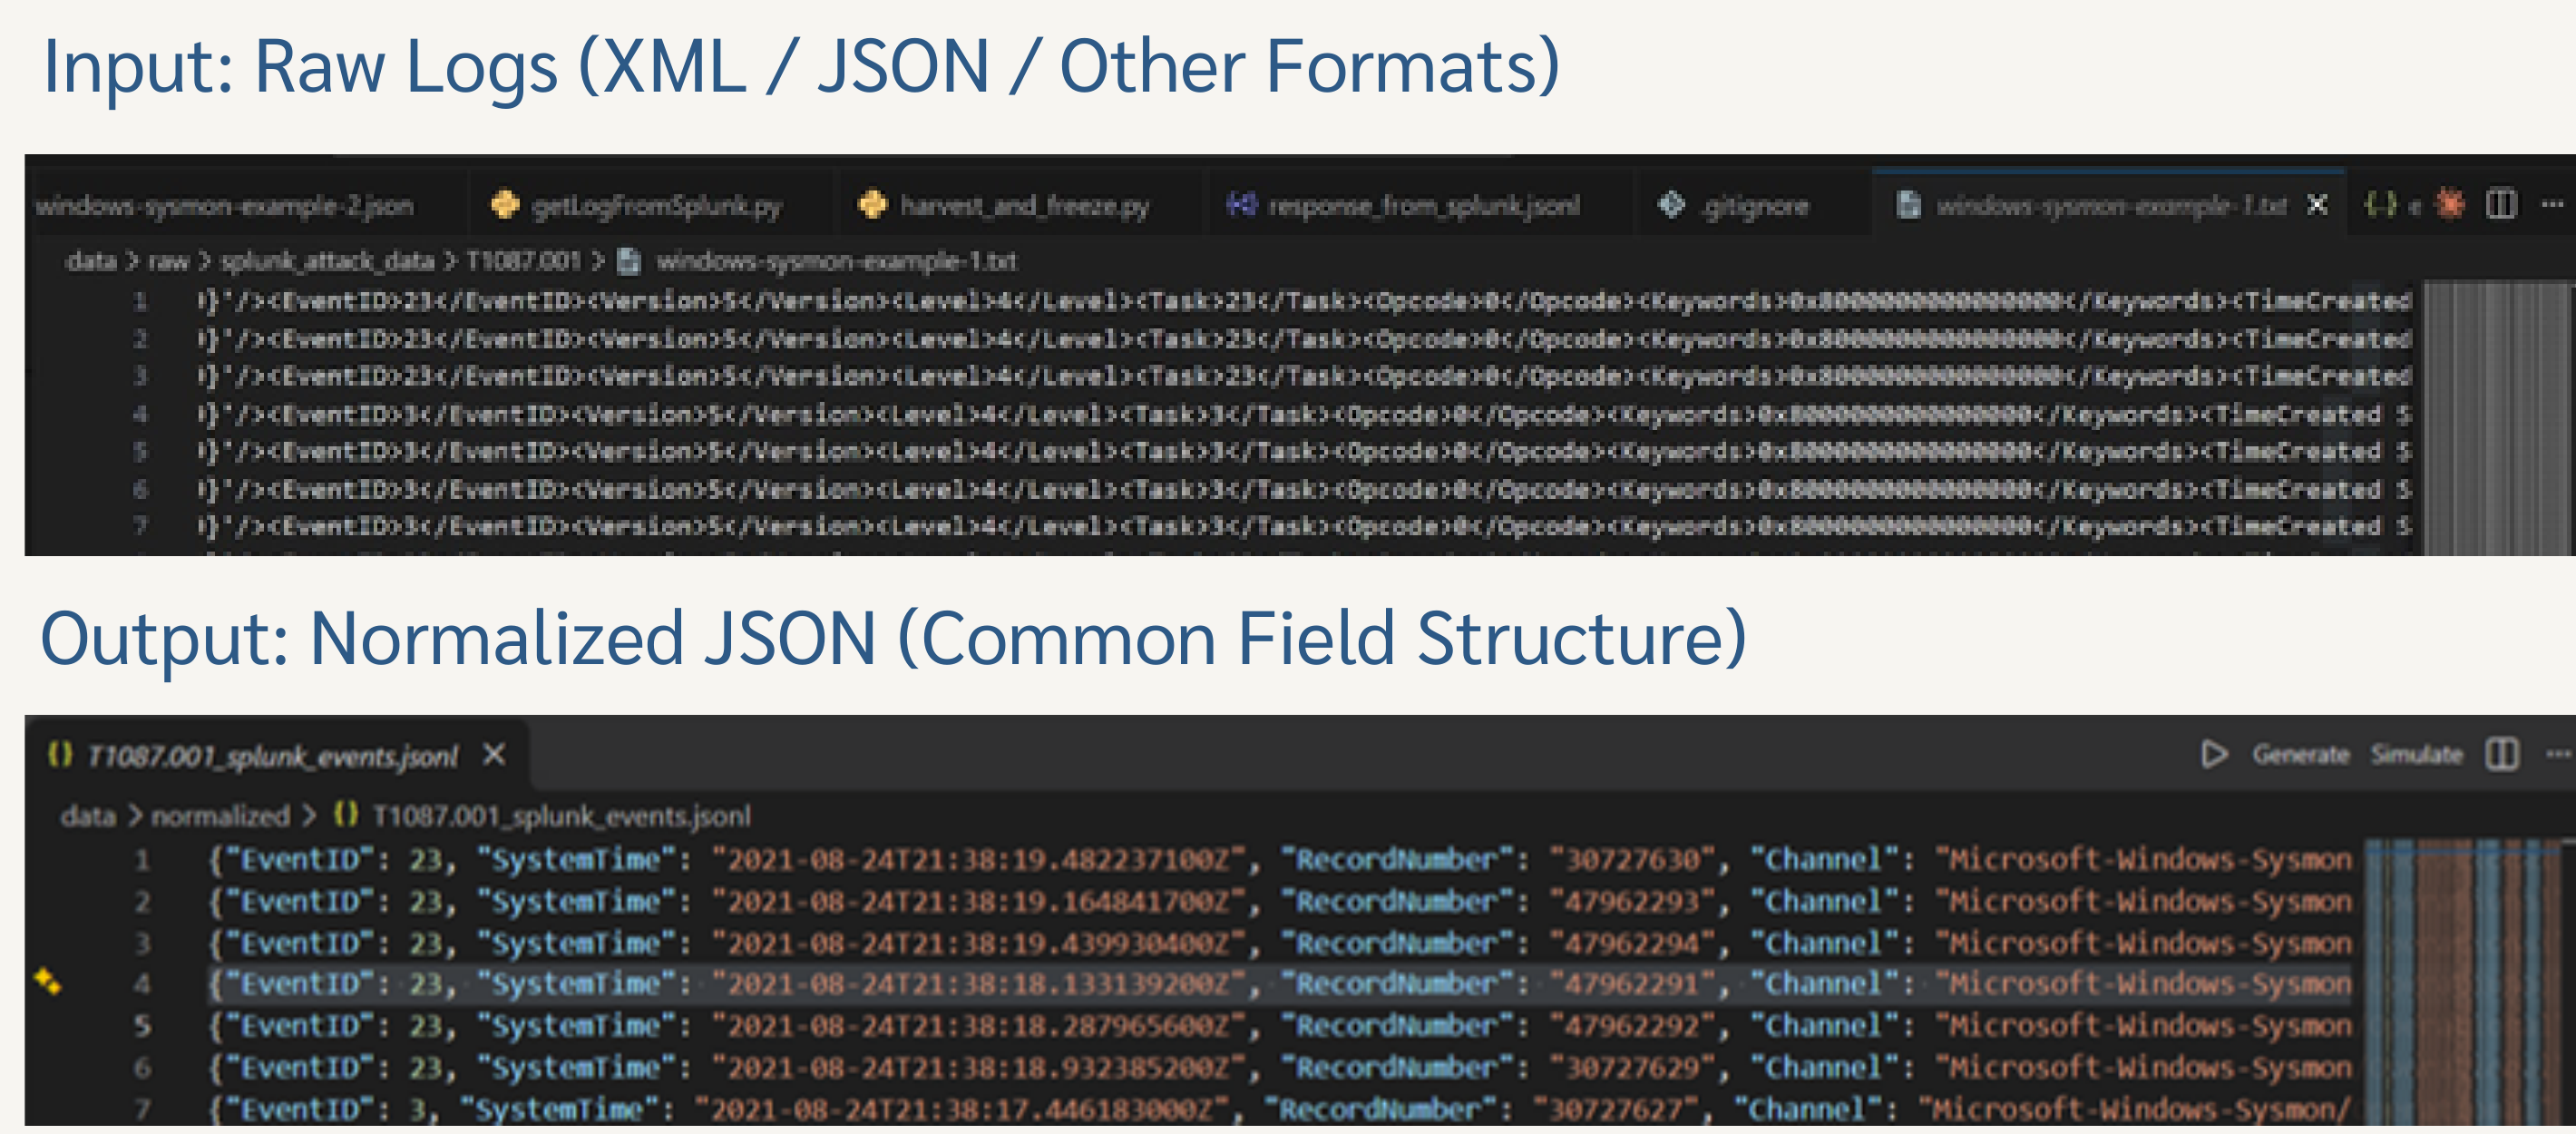
\includegraphics[width=\textwidth]{normalize_example.png}
  \caption{ตัวอย่าง Raw Logs (XML) และผลลัพธ์หลัง Normalize เป็น JSON}
  \label{fig:normalize}
\end{figure}

\subsection{ขั้นตอนที่ 3: Event Selection}
\label{sec:step-es}

Event Selection ตอบคำถามว่า \emph{``จะส่งเหตุการณ์ใดให้ LLM''}
ซึ่งเป็นขั้นตอนที่ยากที่สุดของ Pipeline เพราะต้องคัดเลือกให้ได้หลักฐานครบ แต่ไม่มี Noise มากเกินไป
โครงงานเปรียบเทียบวิธี Event Selection 5 วิธี โดย 4 วิธีแรกเป็นแนวทางพื้นฐาน
และวิธีที่ 5 (Top-$k$ Relevant Events) เป็นวิธีที่โครงงานนำเสนอ

\subsubsection{วิธี Event Selection ที่นำมาเปรียบเทียบ}
\label{sec:es-baselines}
แนวคิดของแต่ละวิธีแสดงในรูปที่~\ref{fig:es-methods} และข้อดีข้อเสียสรุปในตารางที่~\ref{tab:es-methods}

\begin{figure}[htbp]
  \centering
  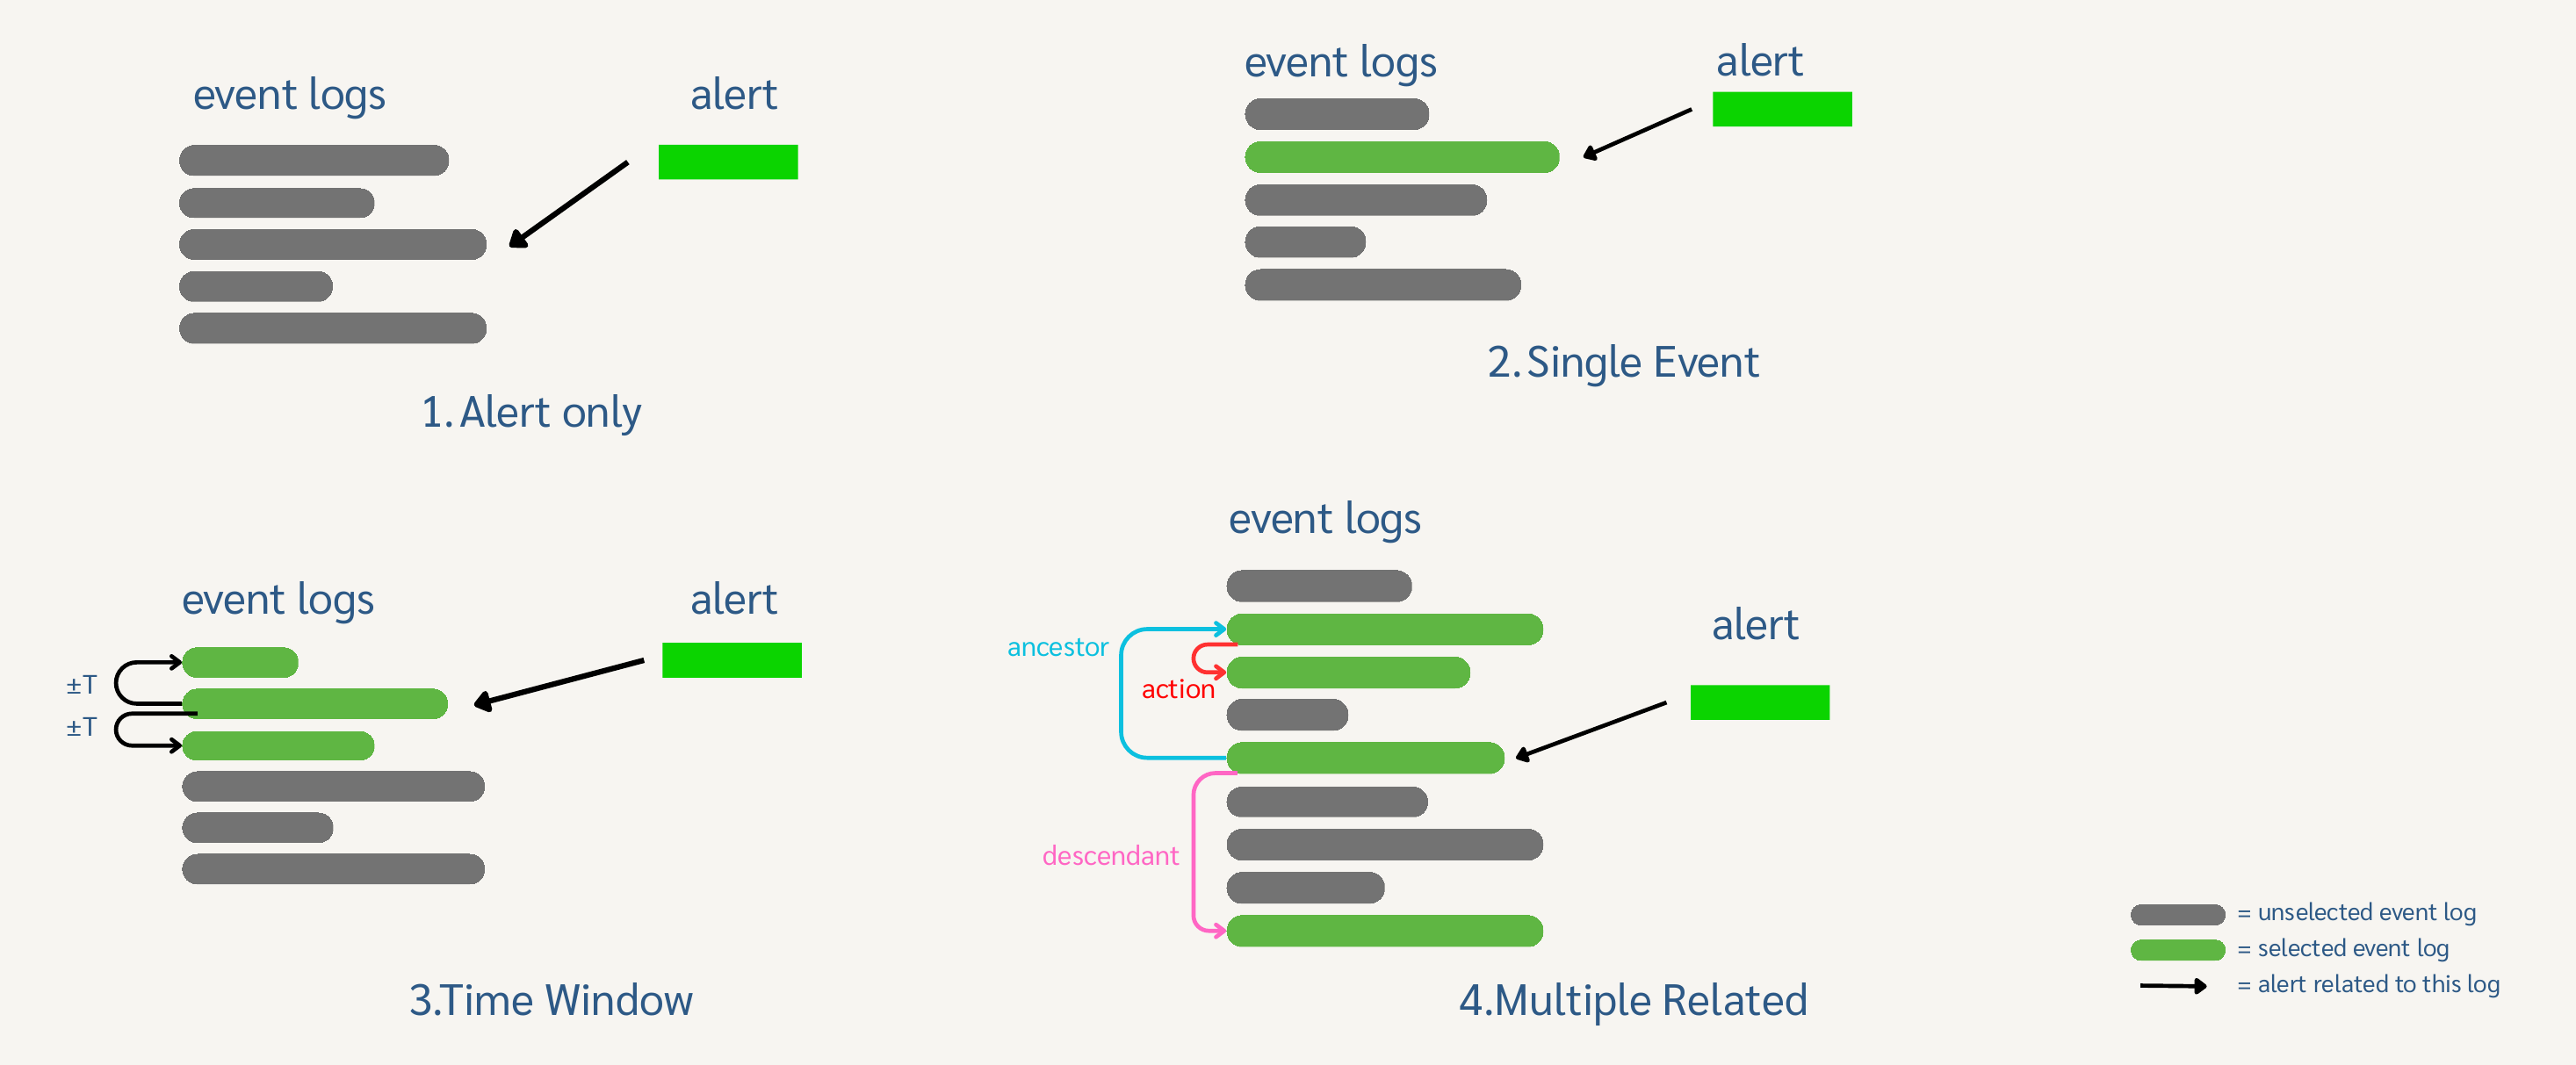
\includegraphics[width=\textwidth]{event_selection_methods.png}
  \caption{แนวคิดของวิธี Event Selection แบบที่ 1--4 (แถบสีเขียวคือ Event ที่ถูกเลือก)}
  \label{fig:es-methods}
\end{figure}

\begin{enumerate}
  \item \textbf{Alert Only} -- ใช้เฉพาะข้อมูลจาก Alert
  \item \textbf{Single Event} -- ดึงเฉพาะ Event เดียวที่ Alert ชี้
  \item \textbf{Time Window} -- ดึง Events ในช่วงเวลา $\pm T$ รอบ Alert
  \item \textbf{Multiple Related Events} -- ดึง Events ที่เชื่อมโยงกันจริงผ่านความสัมพันธ์ของ Process
        (ProcessGuid Lineage) ได้แก่ Ancestor, Descendant และ Events อื่นที่ ProcessGuid เดียวกัน
  \item \textbf{Top-$k$ Relevant Events} -- ให้คะแนนความเกี่ยวข้องกับทุก Event ในขอบเขตที่กำหนด
        แล้วเลือกเฉพาะ Events ที่มีคะแนนสูงสุดภายใต้งบประมาณ Token
\end{enumerate}

\begin{table}[htbp]
  \centering
  \caption{ข้อดีและข้อเสียของวิธี Event Selection แต่ละแบบ}
  \label{tab:es-methods}
  \begin{tabular}{|L{0.16\textwidth}|L{0.36\textwidth}|L{0.36\textwidth}|}
    \hline
    \textbf{วิธี} & \textbf{ข้อดี} & \textbf{ข้อเสีย} \\ \hline
    Alert Only &
      ประมวลผลเร็วที่สุด ไม่มี Overhead จากการ Query และใช้ได้แม้ไม่มี Raw Logs &
      ขาดหลักฐานเชิงลึก ไม่สามารถทำ Evidence Grounding ได้ LLM ได้แต่เชื่อตาม Alert \\ \hline
    Single Event &
      ได้รายละเอียดเต็มของ Event (CommandLine, GUID) และแยกผลของ ``รายละเอียด 1 Event'' ได้ชัด &
      ไม่เห็นว่า Event มาจากไหนหรือต่อไปทำอะไร พลาด Attack Chain ที่กระจายหลาย Event \\ \hline
    Time Window &
      Implement ง่าย (Range Query) ใช้ได้กับ Logs ทุกประเภท และจับ Events ที่เกิดพร้อมกันแต่ไม่เชื่อมกันทางโครงสร้างได้ &
      Noise สูงถ้า $T$ กว้าง พลาด Event ถ้า $T$ แคบ และไม่มีค่า $T$ ที่ถูกต้องสากล \\ \hline
    Multiple Related &
      สร้าง Attack Chain ได้ และตัด Events ที่เกิดพร้อมกันโดยบังเอิญออก &
      พึ่งพา Relationship Key สูง อาจพลาดพฤติกรรมที่ไม่เชื่อมทาง Process และเสี่ยง Over-traversal หากไม่จำกัดความลึก \\ \hline
    Top-$k$ Relevant &
      ควบคุมขนาด Context ได้ (Predictable Context Size) ยืดหยุ่น ปรับ $k$ ตามข้อจำกัด Token ได้ &
      ต้องออกแบบ Scoring Model ให้เป็น Generic และอ่อนไหวต่อค่า $k$ \\ \hline
  \end{tabular}
\end{table}

\FloatBarrier

\subsubsection{วิธีที่เสนอ: Top-$k$ Relevant Events}
\label{sec:topk}
จากตัวอย่าง T1087.001 เมื่อกำหนดให้ Alert ชี้ที่ Process \texttt{net.exe} (คำสั่ง \texttt{net users})
และใช้วิธี Multiple Related เพื่อดึง Process ที่เกี่ยวข้อง (ผู้ใช้ที่รัน, Parent และ Child Process)
พร้อม Events ที่ Process เหล่านั้นเป็นเจ้าของ จำนวน Events ลดลงจาก 11,090 เหลือ 177 Events
แต่จำนวน Events ที่ได้ยังขึ้นกับขนาดของ Process Tree และไม่มีการจัดลำดับความสำคัญ
วิธี Top-$k$ Relevant Events จึงต่อยอดจากแนวคิดนี้โดยให้คะแนนแต่ละ Event และคัดเลือกภายใต้งบประมาณ Token
แบ่งเป็น 4 ขั้นตอนย่อย ได้แก่ (i) Graph (ii) Traverse (iii) Score และ (iv) Budget ดังนี้

\topkstep{i. Graph -- สร้างกราฟความสัมพันธ์ของ Process}
สร้างกราฟความสัมพันธ์ระหว่าง Process และ Event โดยมีโหนดเป็น Process (ระบุด้วย ProcessGuid)
และเส้นเชื่อม 3 ประเภท ดังตารางที่~\ref{tab:graph-edges}
ทุก Event ถูกแนบกับโหนดของ Process เจ้าของ เมื่อการท่องกราฟไปถึงโหนดใดจะได้ Events ทั้งหมดของโหนดนั้น
ส่วน Process ที่ปรากฏเป็น Parent แต่ไม่มี EID 1 ในไฟล์ Log จะถูกตั้งเป็นโหนด Boundary ซึ่งเป็นจุดหยุดการท่องกราฟ

\begin{table}[ht]
  \centering
  \caption{ประเภทเส้นเชื่อมในกราฟความสัมพันธ์ของ Process}
  \label{tab:graph-edges}
  \small
  \begin{tabular}{|l|L{0.32\textwidth}|c|c|}
    \hline
    \textbf{เส้นเชื่อม} & \textbf{สร้างจาก} & \textbf{ใช้ท่องกราฟ} & \textbf{ระยะ (Cost)} \\ \hline
    Parent--Child & EID 1: \texttt{ParentProcessGuid} $\rightarrow$ \texttt{ProcessGuid} & ใช่ & 1 \\ \hline
    File--Exec & EID 11 ของ Process A สร้างไฟล์ X แล้ว EID 1 ของ Process B รันไฟล์ X & ใช่ & 1 \\ \hline
    Process Access & EID 10: Source $\rightarrow$ Target & ไม่ใช่ (แนบเป็นหลักฐาน) & 2 \\ \hline
  \end{tabular}
\end{table}

\noindent
Process Access (EID 10) ไม่ถูกใช้เป็นเส้นทางเดิน เนื่องจากมีสัดส่วนสูงใน Logs และส่วนใหญ่เป็นกิจกรรมปกติของระบบปฏิบัติการ
แต่จะถูกแนบเป็น Candidate ของโหนดที่เดินถึงแล้ว เพื่อให้ยังเห็นพฤติกรรมสำคัญ เช่น การเข้าถึงหน่วยความจำของ \texttt{lsass.exe}

\topkstep{ii. Traverse -- ท่องกราฟจากจุดที่ Alert ชี้}
\label{sec:traverse}
เริ่มจาก Process ที่ Alert ชี้ (Anchor) แล้วขยายไปยัง Parent และ Child Process
โดยเก็บเฉพาะบรรพบุรุษและลูกหลานโดยตรงที่อยู่ในระยะที่กำหนด
เพื่อให้ได้ Candidate Events ที่เกี่ยวข้องกับ Alert โดยไม่ลามไปทั้งระบบ ตามกฎดังนี้
\begin{enumerate}
  \item เดินตามเส้นเชื่อม Parent--Child และ File--Exec โดยหาเส้นทางที่มีระยะรวมน้อยที่สุด (Dijkstra)
  \item เดินทางเดียว คือขึ้นตรงหรือลงตรง ไม่เลี้ยวเข้ากิ่งข้างเคียง
  \item หยุดเมื่อครบจำนวน Hop สูงสุด หรือเจอ Boundary
        (Process ที่รู้ว่ามีอยู่ แต่ไม่มี EID 1 หรือบันทึกการเกิดในไฟล์ Log)
  \item ทุก Process ที่เดินถึง จะเก็บทุก Event ที่ Process นั้นเป็นเจ้าของ
\end{enumerate}
รูปที่~\ref{fig:traverse} แสดงส่วนหนึ่งของกราฟที่ได้จาก Sysmon Log ของ T1087.001
โดยเส้นทึบสีดำคือความสัมพันธ์ Parent--Child (EID 1) และเส้นประสีแดงคือ Process Access (EID 10)

\begin{figure}[ht]
  \centering
  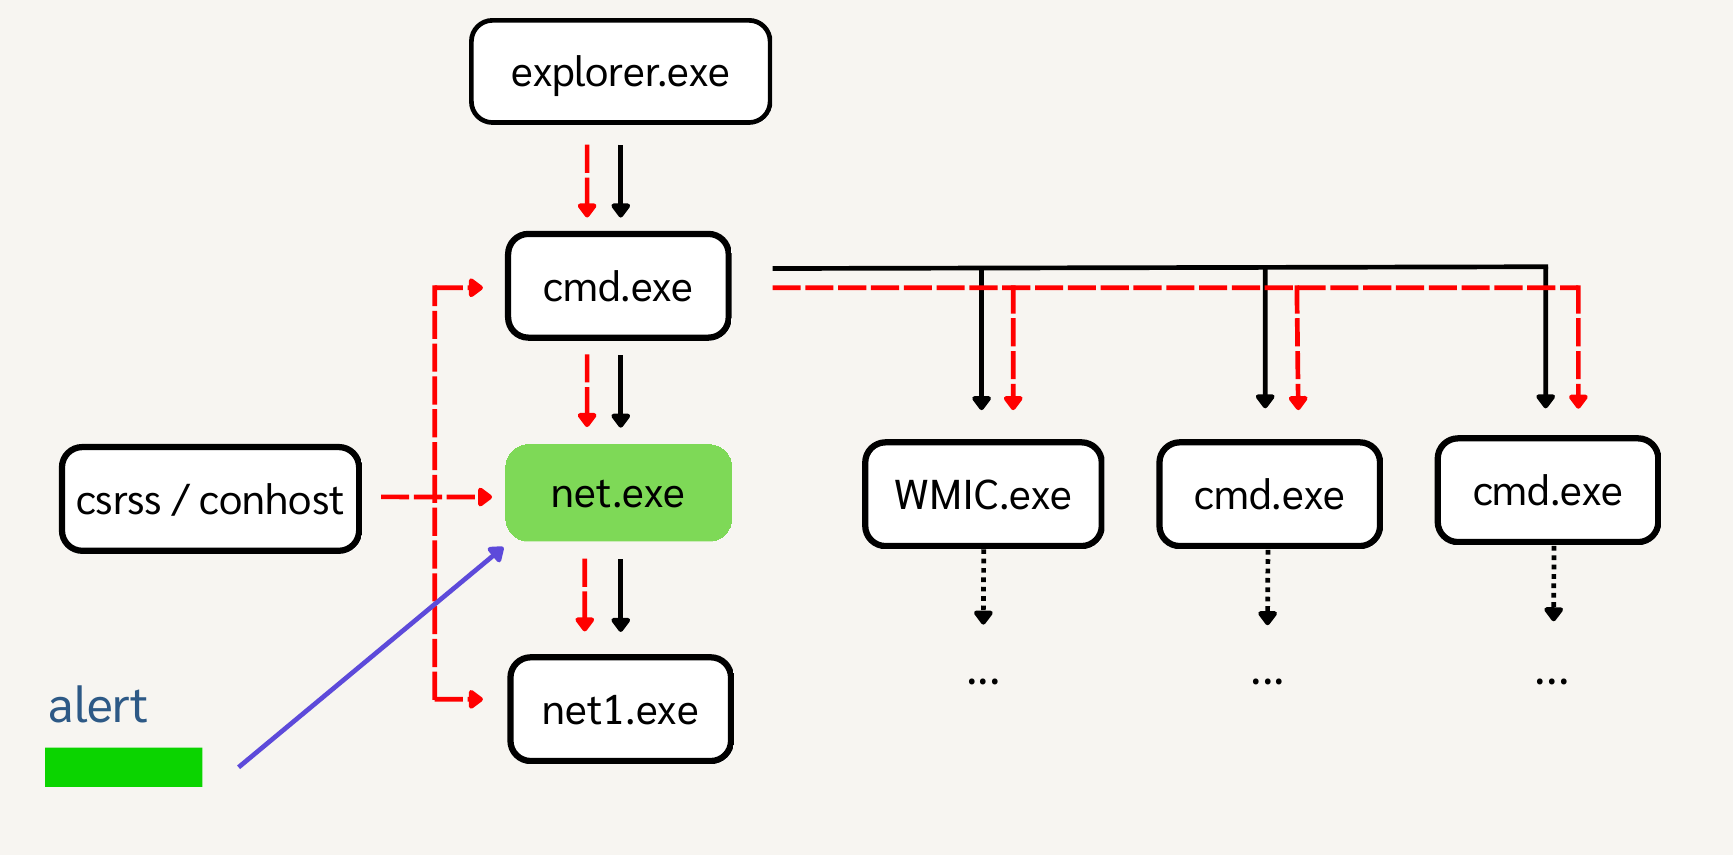
\includegraphics[width=0.85\textwidth]{traverse_graph.png}
  \caption{ส่วนหนึ่งของกราฟ Process จาก Sysmon Log ของ T1087.001 โดยมี \texttt{net.exe} เป็นจุดเริ่ม (Anchor)}
  \label{fig:traverse}
\end{figure}

การท่องกราฟขึ้นกับว่า Anchor มีสายความสัมพันธ์ของ Process (Lineage) หรือไม่ ซึ่งแบ่งได้เป็น 3 กรณี
\begin{enumerate}
  \item[A.] Anchor เป็น EID 1 และมี Lineage (เช่น \texttt{net.exe} ในกรณีนำร่อง) -- ท่องกราฟได้ตามปกติ
  \item[B.] Anchor ไม่ใช่ EID 1 แต่ Process เจ้าของมี EID 1 (เช่น Alert ชี้ EID 13 ของ \texttt{reg.exe})
        -- หาโหนดจาก ProcessGuid แล้วท่องกราฟต่อได้
  \item[C.] Process ของ Anchor ไม่มี EID 1 หรือทั้งไฟล์ไม่มี EID 1
        -- ไม่มีเส้น Parent--Child ให้เดินต่อ ได้เพียง Events ของ Process เดียวและ Events ที่แนบผ่าน EID 10
\end{enumerate}
สำหรับกรณี C จะกำหนดกติกาสำรองก่อนการปรับพารามิเตอร์ แนวทางที่พิจารณาคือ
เพิ่ม Events ในช่วงเวลา $\pm T$ บนเครื่องเดียวกันเป็น Candidate โดยกำหนดระยะเท่ากับจำนวน Hop สูงสุดบวกหนึ่ง
Events เหล่านี้จึงได้คะแนนต่ำกว่า Events ที่เชื่อมกันจริงเสมอ แต่ยังใช้เติมงบประมาณได้
ทุกกรณีทดสอบจะบันทึกว่าอยู่ในกรณี A, B หรือ C และรายงานผลแยกกลุ่ม
เพื่อแสดงว่าวิธี Top-$k$ ทำงานได้แย่ลงเพียงใดเมื่อไม่มี Lineage

\topkstep{iii. Score -- ให้คะแนนความเกี่ยวข้อง}
\textbf{หมายเหตุ:} สมการและค่าพารามิเตอร์ในขั้นนี้เป็นต้นแบบ (Prototype) และค่าเริ่มต้น
ที่ตั้งจากการวิเคราะห์กรณีนำร่อง T1087.001 เท่านั้น ยังไม่ใช่รูปแบบและค่าสุดท้าย
คณะผู้จัดทำจะปรับจูนทั้งรูปแบบของสมการและค่าพารามิเตอร์บน Development Set ภายหลัง
แล้วล็อกค่าก่อนนำไปใช้กับ Test Set

ประเมินและจัดลำดับความเกี่ยวข้องของแต่ละ Candidate Event $e$ ด้วยผลคูณของ 3 ปัจจัย ดังสมการ~\eqref{eq:score}

\begin{equation}\label{eq:score}
\mathrm{Score}(e) = \mathrm{Prox}(e) \times \mathrm{Type}(e) \times \mathrm{Time}(e)
\end{equation}
\begin{align}
\mathrm{Prox}(e) &= \gamma^{\,hop(e)} \\
\mathrm{Type}(e) &= w[\mathrm{EventID}] \\
\mathrm{Time}(e) &= e^{-|\Delta t|/\tau}
\end{align}

\noindent
โดยที่ $hop(e)$ คือจำนวนขั้นบนกราฟจากจุดที่ Alert ชี้ถึง Process เจ้าของ Event,
$\gamma$ คือสัดส่วนคะแนนที่เหลือเมื่อห่างออกไป 1 Hop,
$w[\mathrm{EventID}]$ คือน้ำหนักของ Event แต่ละชนิด (0--1) ที่บอกว่า Event ชนิดนั้นช่วยการวิเคราะห์ได้มากเพียงใด,
$\Delta t$ คือเวลาที่ห่างจาก Alert (วินาที) และ $\tau$ คือช่วงเวลาที่คะแนนลดลงเหลือประมาณ $1/e$ (ราว $1/3$)
ค่าเริ่มต้นของพารามิเตอร์แสดงในตารางที่~\ref{tab:score-param}
และตัวอย่างการคำนวณคะแนนแสดงในตารางที่~\ref{tab:score-example}

การรวมปัจจัยแบบผลคูณทำให้ Event ที่มีปัจจัยใดปัจจัยหนึ่งต่ำได้คะแนนต่ำโดยรวม
แนวทางการปรับจูนที่จะทดลองบน Development Set ได้แก่ การเปรียบเทียบกับรูปแบบอื่น
เช่น การรวมแบบผลรวมถ่วงน้ำหนัก (Weighted Sum) การตัดปัจจัยใดปัจจัยหนึ่งออกเพื่อดูผลของแต่ละปัจจัย (Ablation)
และวิธีนับระยะของ Events ที่แนบผ่าน Process Access
โดยใช้ Evidence Recall และความถูกต้องของ LLM บน Development Set เป็นเกณฑ์เลือก
ก่อนล็อกค่าและนำไปใช้กับ Test Set

\begin{table}[ht]
  \centering
  \caption{ค่าพารามิเตอร์เริ่มต้นของการให้คะแนน (จะปรับจูนบน Development Set ภายหลัง)}
  \label{tab:score-param}
  \begin{tabular}{|c|c|l|}
    \hline
    \textbf{พารามิเตอร์} & \textbf{ค่า} & \textbf{ความหมาย} \\ \hline
    $\gamma$ & 0.6 & Hop 0 = 1, Hop 1 = 0.6, Hop 2 = 0.36 \\ \hline
    $w[\text{EID 1}]$ & 1.0 & Process Creation มีข้อมูลคำสั่งครบ \\ \hline
    $w[\text{EID 10}]$ & 0.2 & Process Access ให้ข้อมูลประกอบ \\ \hline
    $\tau$ & 300 วินาที & ห่าง 300 วินาที คะแนนเวลาเหลือ 0.37 \\ \hline
  \end{tabular}
\end{table}

\begin{table}[ht]
  \centering
  \caption{ตัวอย่างการคำนวณคะแนนของ Candidate Events จาก T1087.001}
  \label{tab:score-example}
  \begin{tabular}{|l|c|c|c|c|c|c|}
    \hline
    \textbf{Event} & \textbf{Hop} & \textbf{$\Delta t$} & \textbf{Prox} & \textbf{Type} & \textbf{Time} & \textbf{Score} \\ \hline
    net1.exe (EID 1)         & 1 & 0.01 s & 0.6 & 1.0 & 1.00 & 0.60 \\ \hline
    cmd.exe (EID 1)          & 1 & 6.6 s  & 0.6 & 1.0 & 0.98 & 0.59 \\ \hline
    net $\rightarrow$ net1 (EID 10) & 0 & 0 s & 1.0 & 0.2 & 1.00 & 0.20 \\ \hline
    cmd $\rightarrow$ WMIC (EID 10) & 1 & 11 s & 0.6 & 0.2 & 0.97 & 0.12 \\ \hline
    cmd $\rightarrow$ cmd (EID 10)  & 1 & 74 s & 0.6 & 0.2 & 0.78 & 0.09 \\ \hline
  \end{tabular}

  \vspace{1mm}
  {\footnotesize หมายเหตุ: ค่า Hop ของ Events ชนิด EID 10 ในตารางนี้คำนวณด้วยวิธีนับ Hop แบบเดิม
  ซึ่งยังไม่ได้ใช้ระยะ (Cost) ตามตารางที่~\ref{tab:graph-edges}
  วิธีนับระยะของ EID 10 จะปรับในการทดลองขั้นต่อไป\par}
\end{table}

\topkstep{iv. Budget -- คัดเลือกภายใต้งบประมาณ Token}
เพื่อจำกัดจำนวน Token ให้พอดีกับ Context Window ของโมเดล และให้ LLM เห็นเฉพาะ Events ที่สำคัญที่สุดก่อน
ขั้นตอน Budget ทำงาน 3 ข้อ ดังนี้
\begin{enumerate}
  \item ใส่ Event ที่ Alert ชี้ (Anchor) เป็นอันดับแรก
  \item เรียง Events ที่เหลือตามคะแนนจากมากไปน้อย
  \item ใส่ทีละ Event พร้อมนับจำนวน Token สะสม หากเกินโควตา $B$ ให้หยุด
\end{enumerate}
ตัวอย่างเช่น หากกำหนดโควตา $B = 400$ Tokens และแต่ละ Event ใช้ประมาณ 100--130 Tokens
จะมีเพียงประมาณ 3 Events แรกเท่านั้นที่ถูกส่งต่อไปยังขั้นตอนถัดไป

\subsection{ขั้นตอนที่ 4: Representation}
\label{sec:step-rep}

Representation ตอบคำถามว่า \emph{``จะนำเสนอ Logs ที่คัดเลือกแล้วให้ LLM ในรูปแบบใดจึงเหมาะสมที่สุด''}
เนื่องจากข้อมูลชุดเดียวกันเขียนต่างรูปแบบกันจะได้จำนวน Token และความเข้าใจของ LLM ที่ต่างกัน
โครงงานเปรียบเทียบ 5 รูปแบบ (รูปที่~\ref{fig:representation} และตารางที่~\ref{tab:representation})
โดยพิจารณาตามลำดับความสำคัญ คือ (1) Accuracy ในการระบุเทคนิค และ (2) Token Efficiency

\begin{figure}[ht]
  \centering
  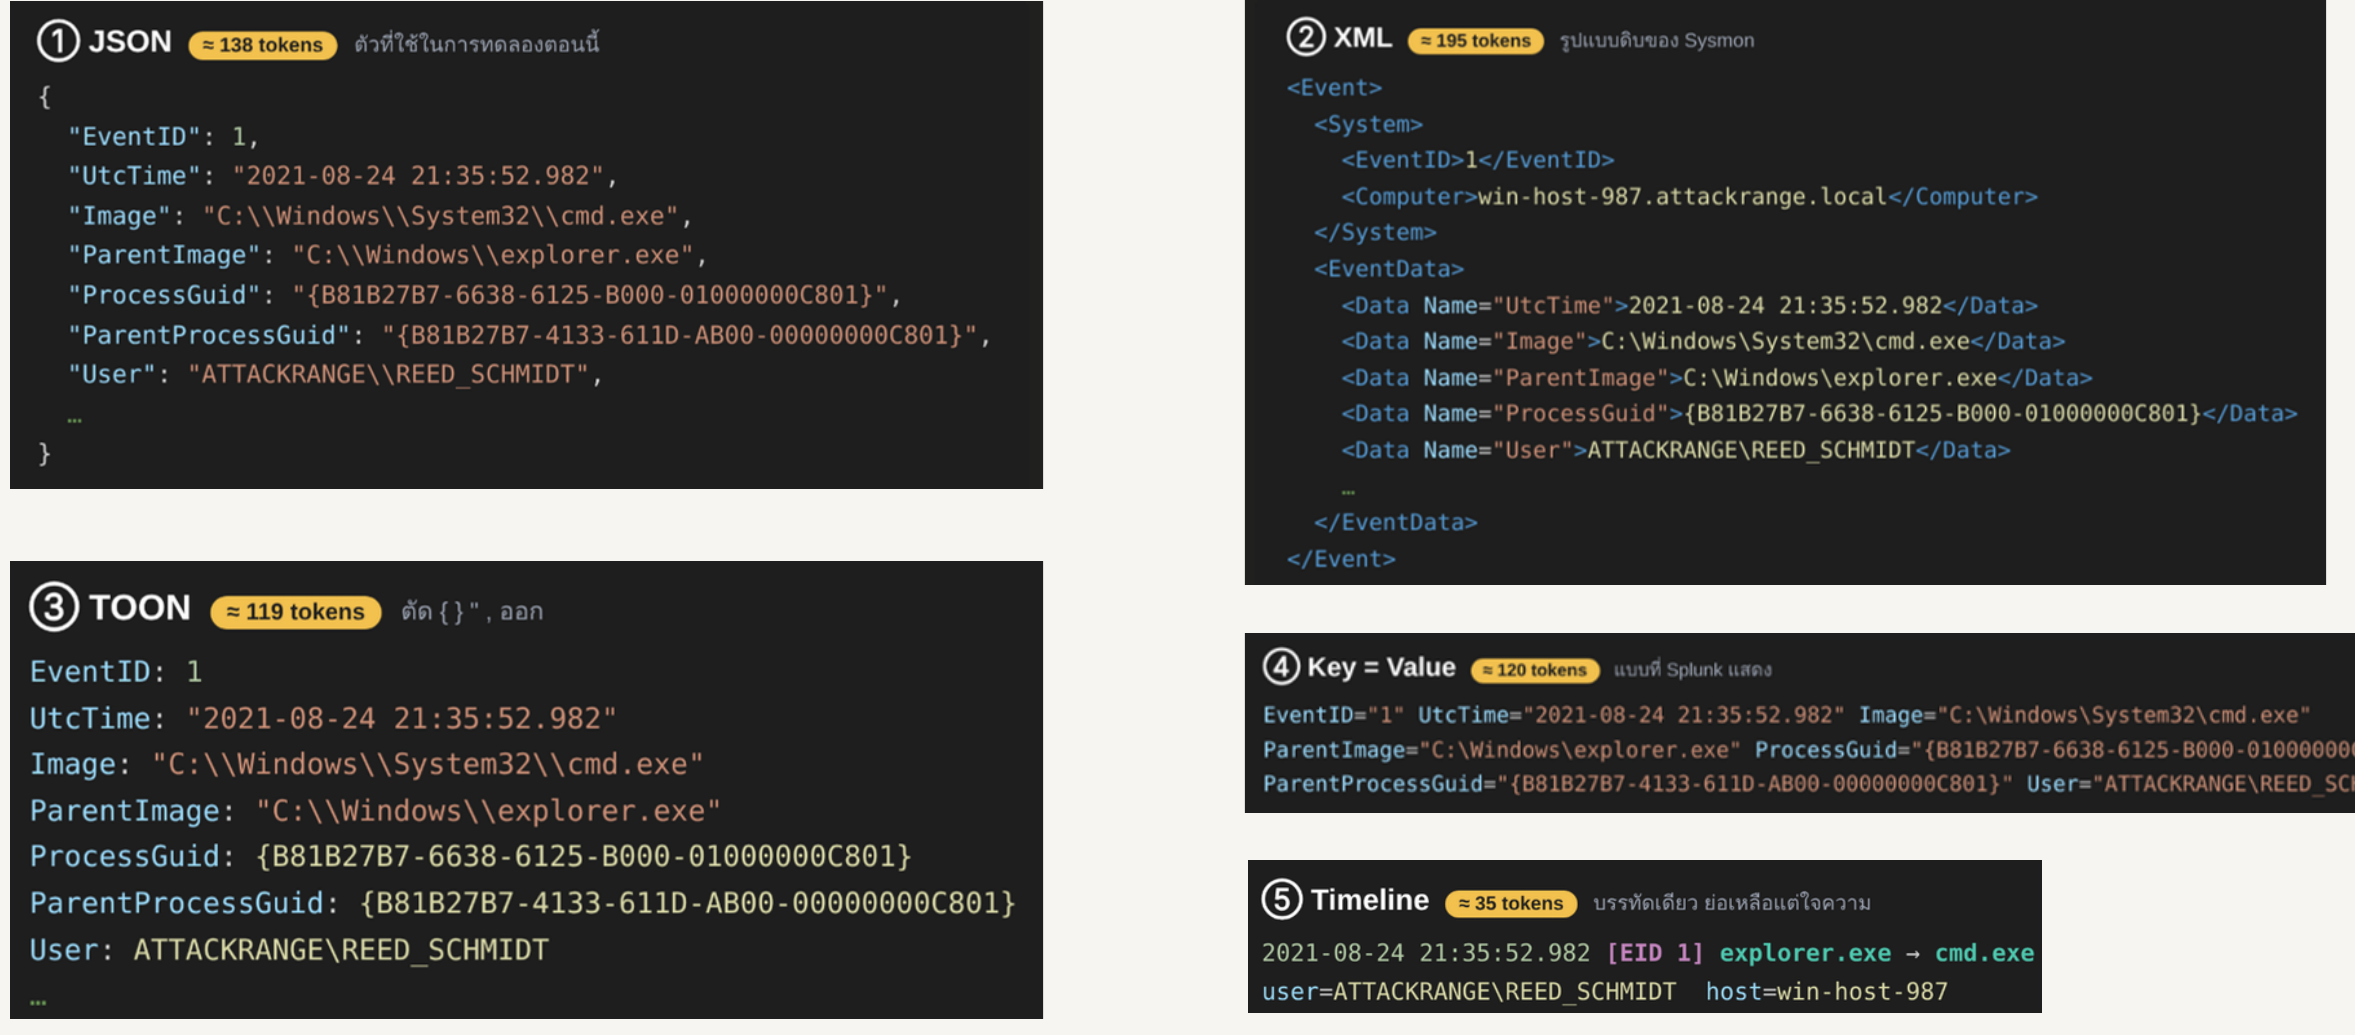
\includegraphics[width=\textwidth]{representation_formats.png}
  \caption{ตัวอย่าง Event เดียวกันในรูปแบบ JSON, XML, TOON, Key=Value และ Timeline}
  \label{fig:representation}
\end{figure}

\begin{table}[ht]
  \centering
  \caption{จำนวน Token โดยประมาณของ Event ตัวอย่าง (Sysmon EID 1) ในแต่ละรูปแบบ}
  \label{tab:representation}
  \begin{tabular}{|l|c|l|}
    \hline
    \textbf{รูปแบบ} & \textbf{Tokens (ประมาณ)} & \textbf{ลักษณะ} \\ \hline
    Timeline   & 35  & บรรทัดเดียว กระชับที่สุด แต่ข้อมูลบางส่วนหายไป \\ \hline
    TOON       & 119 & ตัด \{\} และ "" ออกจาก JSON \\ \hline
    Key=Value  & 120 & รูปแบบที่ Splunk แสดงผล \\ \hline
    JSON       & 138 & Output ของขั้นตอน Normalize (ใช้ในการทดลองปัจจุบัน) \\ \hline
    XML        & 195 & รูปแบบต้นฉบับของ Sysmon \\ \hline
  \end{tabular}
\end{table}

ในการทดลองปัจจุบันโครงงานเลือกใช้รูปแบบ JSON เนื่องจากได้มาโดยตรงจากขั้นตอนก่อนหน้า
ส่วนการเปรียบเทียบ Accuracy ระหว่างรูปแบบต่าง ๆ จะดำเนินการในการทดลอง E2 (หัวข้อ~\ref{sec:main-exp})

\subsection{ขั้นตอนที่ 5: Retrieval-Augmented Generation (RAG)}
\label{sec:step-rag}

RAG ทำหน้าที่เพิ่มบริบทให้ LLM โดยอ้างอิงองค์ความรู้จาก MITRE ATT\&CK
ฐานความรู้สร้างจากเอกสาร MITRE ATT\&CK Enterprise v19.2 (STIX ทางการ)
แปลงเป็น JSON และแบ่ง Chunk ตาม Technique และ Sub-technique
(1 Chunk ต่อ 1 Technique หรือ 1 Sub-technique) รวมทั้งหมด 697 Chunks (222 Techniques + 475 Sub-techniques)
ดังรูปที่~\ref{fig:rag-kb}
ข้อความของแต่ละ Chunk ประกอบด้วยชื่อ Tactics และคำอธิบาย (Description) โดยไม่ Embed รหัสเทคนิค
เหตุผลที่แบ่งถึงระดับ Sub-technique คือคำตอบที่ต้องการอยู่ในระดับ Sub-technique
และ Sub-technique ภายใต้ Technique เดียวกันมักต่างกันเพียงในคำอธิบาย
เช่น T1087.001 (\texttt{net user}) กับ T1087.002 (\texttt{net user /domain})
แต่ละ Chunk ถูกแปลงเป็นเวกเตอร์ด้วย \texttt{qwen3-embedding:0.6b} ผ่าน Ollama
ความยาวมัธยฐานของ Chunk ประมาณ 1,100 ตัวอักษร (ประมาณ 280 Tokens)

\begin{figure}[ht]
  \centering
  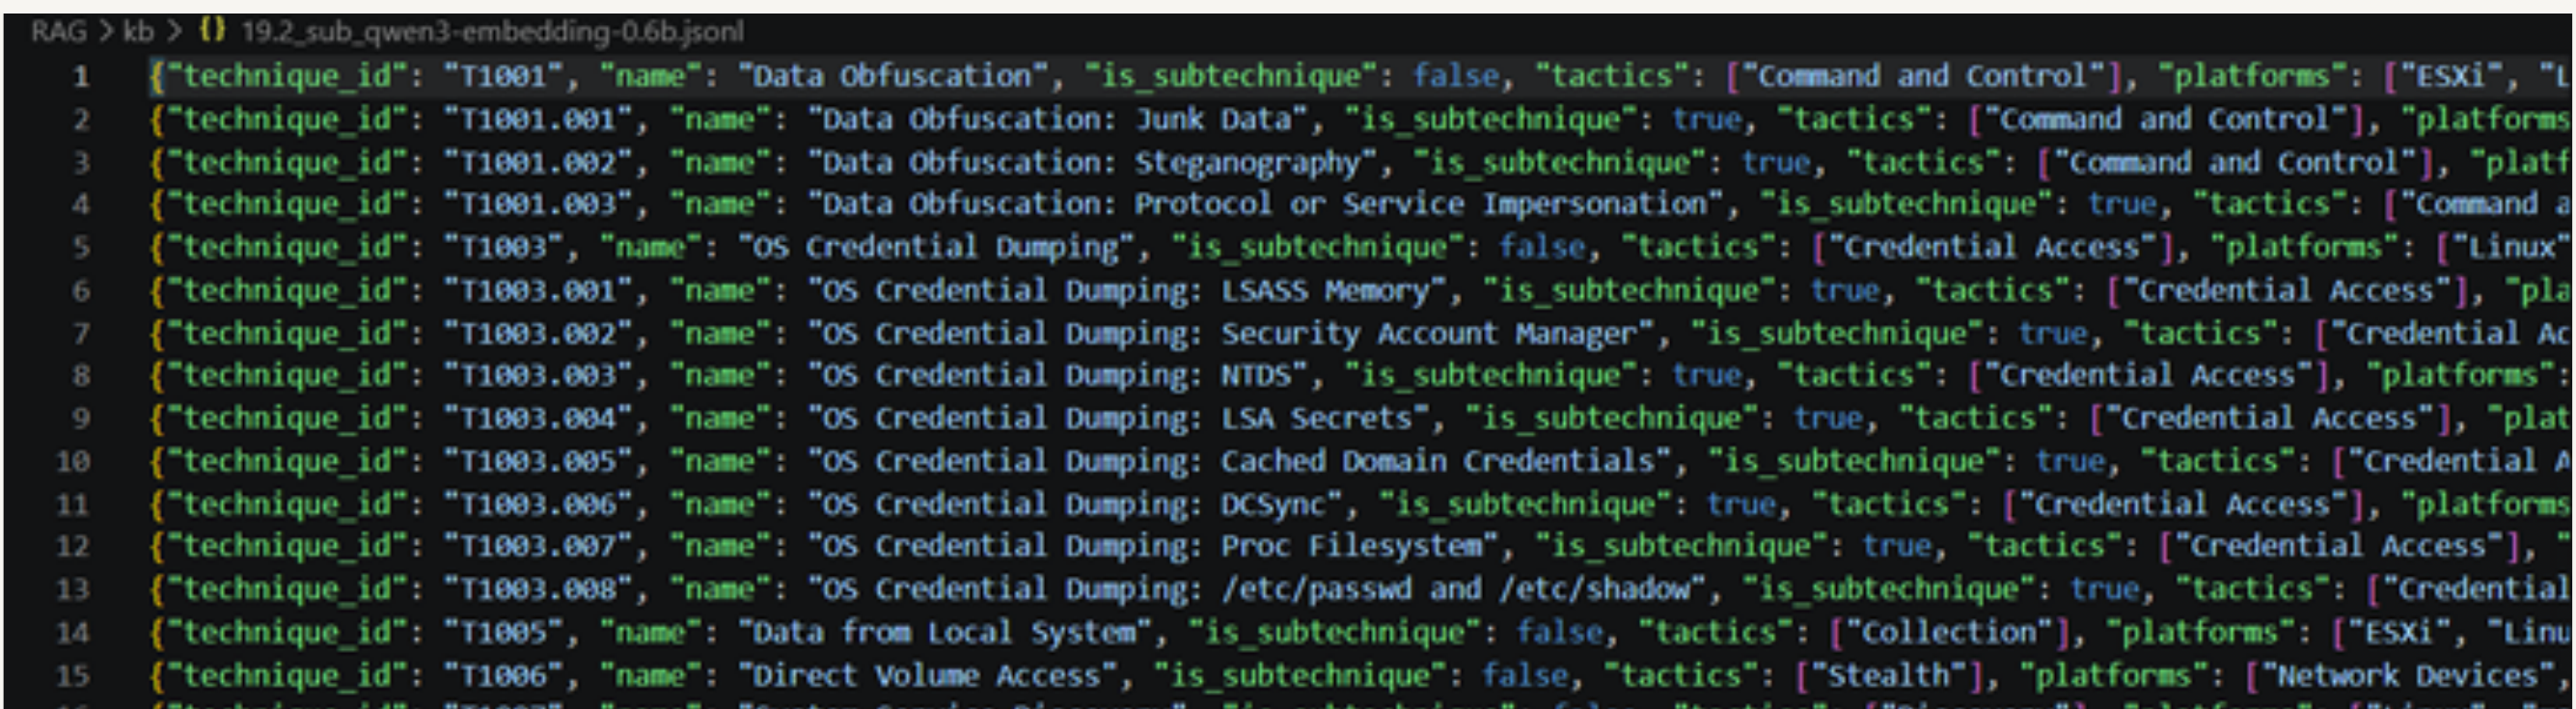
\includegraphics[width=\textwidth]{rag_kb_chunks.png}
  \caption{ตัวอย่างฐานความรู้ MITRE ATT\&CK v19.2 ที่แบ่ง Chunk ตาม Technique และ Sub-technique}
  \label{fig:rag-kb}
\end{figure}

Query ที่ใช้ค้นหาในฐานความรู้มีได้ 2 แบบ คือ
(1) ใช้ Representation Log (JSON) โดยตรง และ
(2) ให้ LLM แปลง Representation Log เป็นคำอธิบายพฤติกรรมภาษาอังกฤษ (Log Summary) ก่อน
โดยห้ามใช้ชื่อหรือรหัสเทคนิค ผลลัพธ์ของ RAG คือรายการ Top-$k$ Techniques ที่ใช้เป็น Context ให้ LLM

\subsection{ขั้นตอนที่ 6: LLM Analysis และ Output}
\label{sec:step-llm}

LLM ที่ใช้คือ Qwen3.5:9B ทำงานภายในเครื่องผ่าน Ollama ร่วมกับ Hermes เป็น Harness
LLM รับ Context จาก RAG และ Representation Log แล้วระบุเทคนิคการโจมตี
Prompt ถูกออกแบบให้ LLM ทำงานเป็นลำดับ ได้แก่
อ่าน Event ที่ Alert ชี้ก่อน $\rightarrow$ พิจารณาว่าคำสั่งทำอะไร $\rightarrow$ ระบุ Technique
$\rightarrow$ ระบุ Sub-technique ที่ตรงกับรูปแบบคำสั่ง $\rightarrow$ ระบุทางเลือกที่ใกล้เคียงและเหตุผลที่ไม่ใช่
และตอบในรูปแบบ JSON ที่มีโครงสร้างกำหนด (เช่น พฤติกรรมที่สังเกตได้ ทางเลือกที่พิจารณา รหัสเทคนิค และความมั่นใจ)
สำหรับกรณีใช้ RAG จะระบุใน Prompt ว่ารายการ Candidate เป็นเพียงคำใบ้ และคำตอบที่ถูกอาจไม่อยู่ในรายการ
การตั้งค่าในการทดลอง ได้แก่ ปิดโหมด Thinking, Temperature = 0 และ Context Window 16,384 Tokens

เพื่อป้องกันการรั่วไหลของเฉลย ระบบจะตรวจสอบว่า Prompt และ Query ไม่มีรหัสเทคนิค
(รูปแบบ \texttt{T\#\#\#\#}) หรือรหัส Case ที่บอกคำตอบ ก่อนส่งให้ LLM
ผลลัพธ์สุดท้ายคือ Investigation Report ที่ระบุเทคนิค ATT\&CK หลักฐาน (Event ที่อ้างอิง) และเหตุผลประกอบ

\section{ต้นแบบ Web Dashboard}
\label{sec:dashboard}

ผลการวิเคราะห์ถูกนำเสนอให้ SOC Analyst ผ่าน Web Dashboard
ซึ่งออกแบบให้รับข้อมูลได้ 2 แบบ คือ อัปโหลดไฟล์ Logs ด้วยตนเอง (Manual Investigation) ซึ่งเป็นแบบที่ใช้ในระยะนี้
และรับ Alert จาก SIEM อัตโนมัติ ซึ่งจะพัฒนาในระยะถัดไป
หน้า Inbox (รูปที่~\ref{fig:dashboard}) แสดงรายการการสืบสวนทั้งหมด พร้อมแหล่งที่มา ความรุนแรง เวลา
ชื่อ Alert และ Host สถานะการประมวลผลของ LLM (Pending, Processing, Analyzed, Failed)
ผลลัพธ์ (เทคนิคที่ระบุได้) และผู้รับผิดชอบ
นอกจากนี้ยังมีเมนูสำหรับผู้ดูแลระบบ เช่น การเชื่อมต่อ SIEM การตั้งค่า Pipeline
และการปรับปรุงข้อมูล/ฐานความรู้ ซึ่งกำหนดให้ผู้ดูแลระบบเป็นผู้สั่งปรับปรุงเท่านั้น

\begin{figure}[htbp]
  \centering
  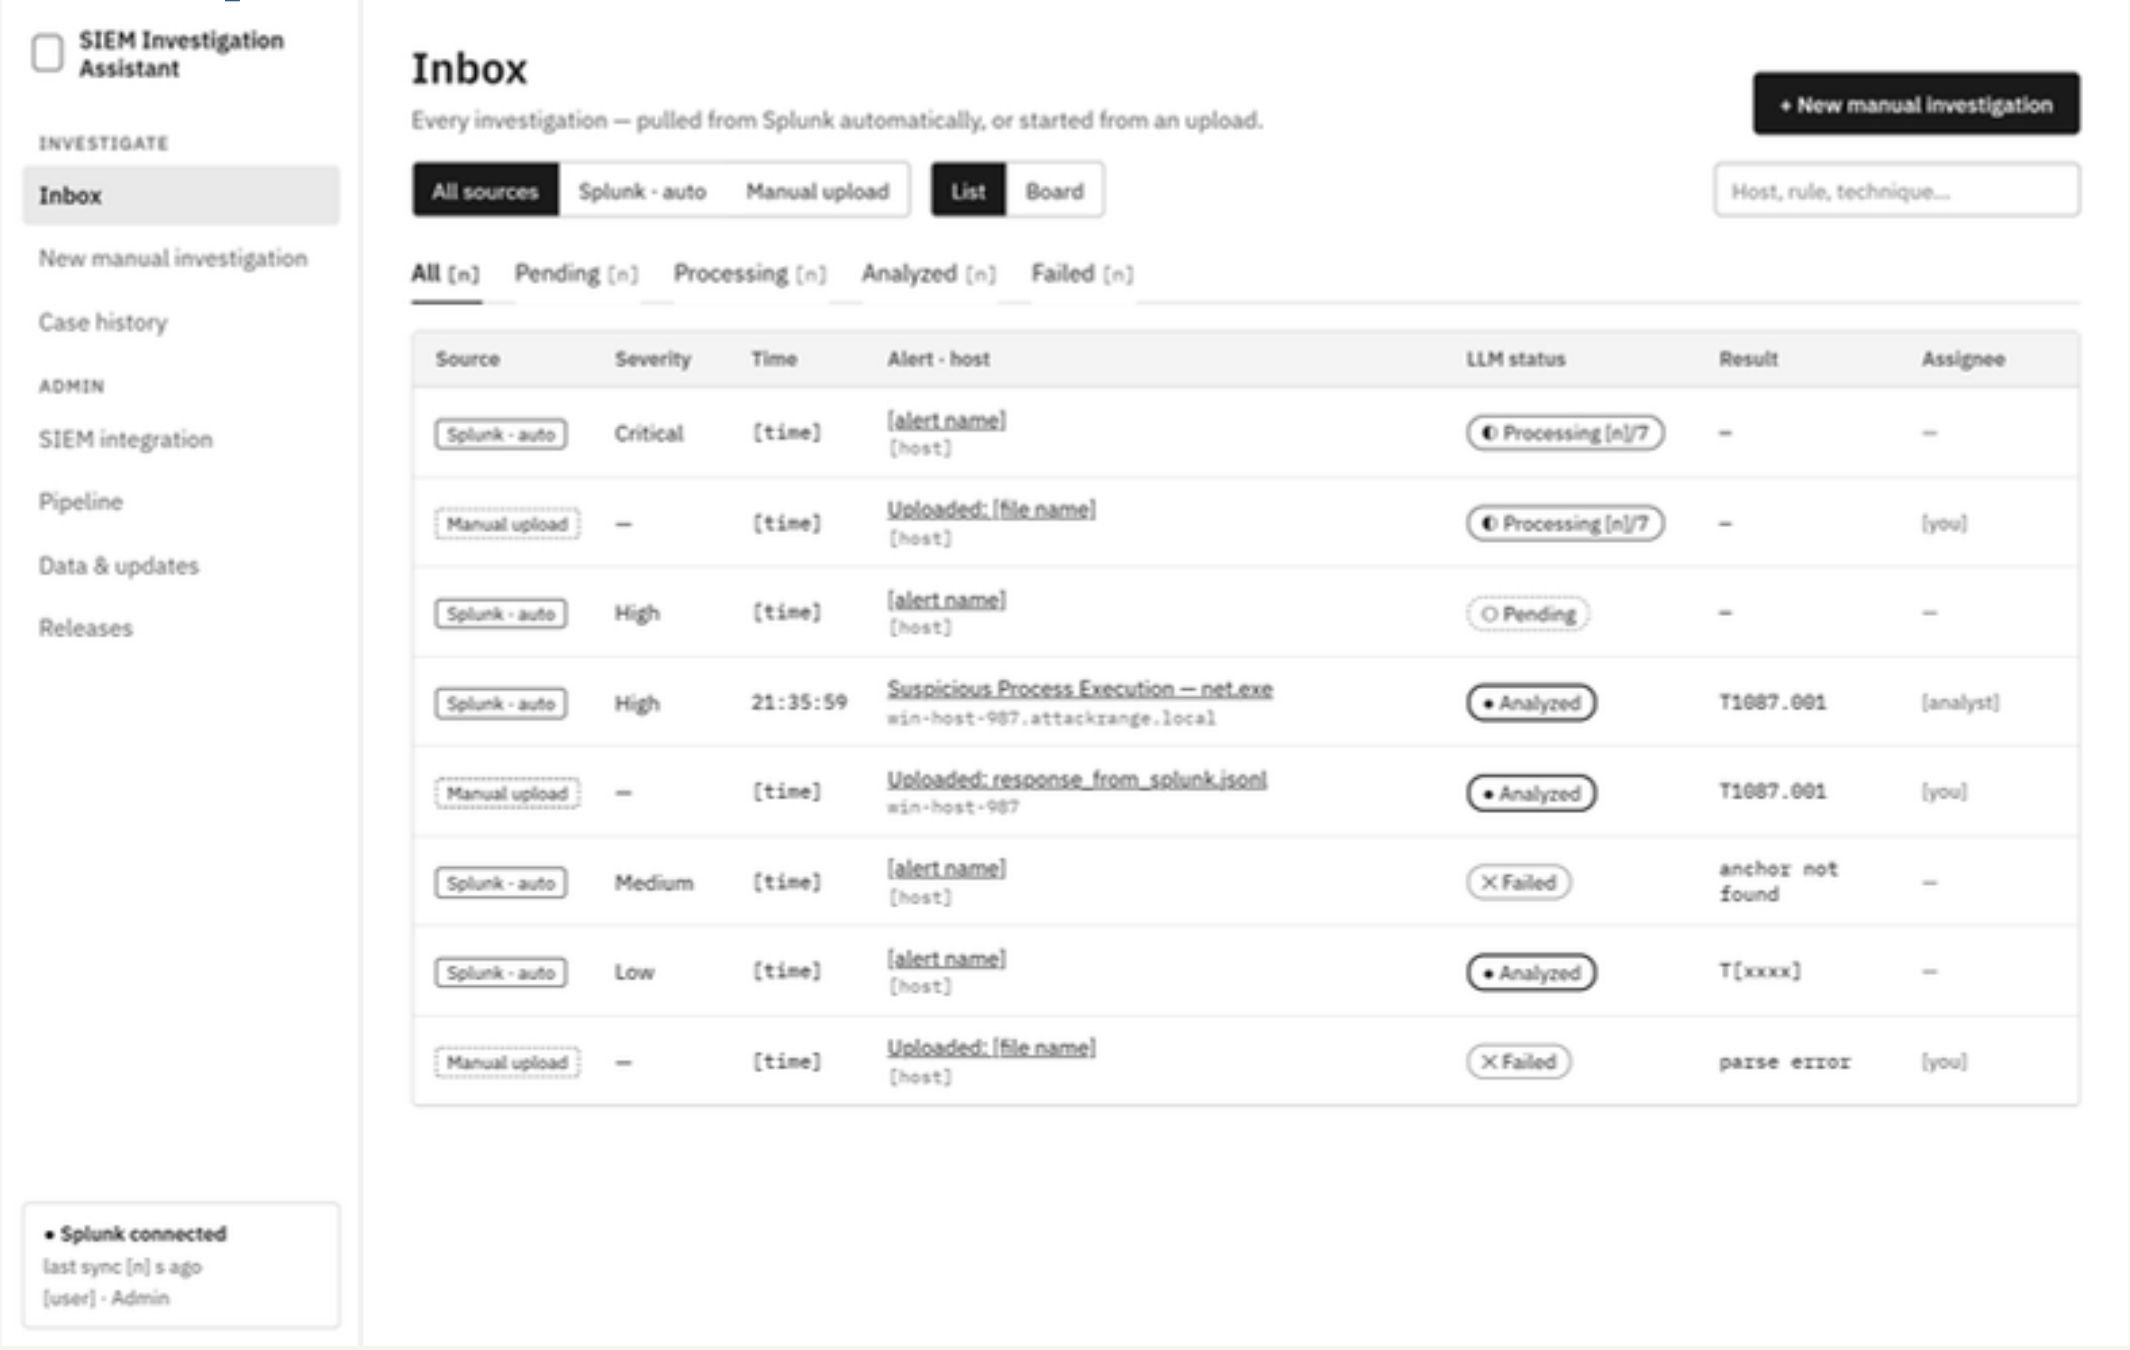
\includegraphics[width=\textwidth]{dashboard_prototype.png}
  \caption{ต้นแบบหน้า Inbox ของ Web Dashboard}
  \label{fig:dashboard}
\end{figure}

\chapter{\ifproject%
\ifenglish Experimentation and Results\else การทดลองและผลลัพธ์\fi
\else%
\ifenglish System Evaluation\else การประเมินระบบ\fi
\fi}

บทนี้นำเสนอการทดลองเบื้องต้นที่ดำเนินการแล้ว 2 การทดลอง ได้แก่
(1) การส่ง Raw Logs ให้ LLM เชิงพาณิชย์วิเคราะห์โดยตรง เพื่อยืนยันปัญหาของโครงงาน และ
(2) การทดลองนำร่องเพื่อตรวจสอบว่า LLM ขนาดเล็กยังจำเป็นต้องใช้ RAG หรือไม่
จากนั้นนำเสนอแผนการทดลองหลัก ตัวชี้วัด ลำดับการดำเนินการ และประเด็นที่ยังเปิดอยู่

\section{การทดลองเบื้องต้น: ส่ง Raw Logs ให้ LLM วิเคราะห์โดยตรง}

\subsection{วิธีการทดลอง}
การทดลองนี้ดำเนินการก่อนการนำเสนอความก้าวหน้าครั้งที่ 1 โดยดึง Windows Sysmon Logs ของชุดข้อมูล T1087.001 จาก Splunk ผ่าน REST API
ได้เป็นไฟล์ JSON Lines จำนวน 11,090 Events (ข้อมูลต้นฉบับในรูปแบบ XML มีขนาดประมาณ 16.8 MB)
ซึ่งมีขนาดใหญ่กว่า Context Window ของ LLM ทั่วไป
แล้วอัปโหลดไฟล์ให้ LLM เชิงพาณิชย์ 3 โมเดลวิเคราะห์โดยตรง
ด้วยคำถามว่า ``นี่คือ Attack Technique อะไร เพราะอะไรถึงคิดแบบนั้น''
คำตอบที่ถูกต้อง (Ground Truth) คือ Account Discovery: Local Account (T1087.001)

\subsection{ผลการทดลอง}
\begin{table}[ht]
  \centering
  \caption{ผลการส่ง Raw Logs ของ T1087.001 ให้ LLM เชิงพาณิชย์วิเคราะห์โดยตรง}
  \label{tab:raw-llm}
  \begin{tabular}{|L{0.25\textwidth}|L{0.45\textwidth}|L{0.17\textwidth}|}
    \hline
    \textbf{โมเดล} & \textbf{คำตอบ} & \textbf{ผลเทียบเฉลย} \\ \hline
    GPT-5.6 Luna      & T1003 OS Credential Dumping & ผิด \\ \hline
    Gemini 3.1 Pro    & ไม่พบพฤติกรรมการโจมตีที่ชัดเจน (Logs เป็นเพียงการทำงานของ Splunk Agent) & ผิด \\ \hline
    Claude Sonnet 5 (High) & T1087 Account Discovery & ถูกเฉพาะระดับ Technique (Parent Match) \\ \hline
  \end{tabular}
\end{table}

จากตารางที่~\ref{tab:raw-llm} พบว่าแม้เป็นโมเดลขนาดใหญ่ แต่เมื่อได้รับ Raw Logs ที่มี Noise จำนวนมาก
บางโมเดลให้ความสำคัญกับ Events ที่ไม่เกี่ยวข้อง เช่น Gemini 3.1 Pro
ที่สรุปว่า Logs เป็นเพียงการทำงานของ Splunk Agent
และไม่มีโมเดลใดระบุ Sub-technique ได้ถูกต้อง
ผลนี้เป็นหลักฐานเบื้องต้นที่สนับสนุนว่าการสร้าง Investigation Context ที่คัดกรองแล้วมีความจำเป็น
ทั้งนี้ การทดลองนี้ทำผ่านหน้าเว็บของแต่ละบริการเพียงครั้งเดียว จึงควบคุมการตั้งค่าของโมเดลไม่ได้
และใช้เพียง 1 กรณี ผลจึงใช้เป็นตัวอย่างประกอบปัญหา ไม่ใช่การเปรียบเทียบความสามารถของโมเดล

\section{การทดลองนำร่อง: ความจำเป็นของ RAG สำหรับ LLM ขนาดเล็ก}

\subsection{วัตถุประสงค์และการตั้งค่า}
การทดลองนี้มีวัตถุประสงค์เพื่อตรวจสอบว่า เมื่อ Input ผ่าน Event Selection แล้ว
LLM ขนาดเล็ก (Qwen3.5:9B) ยังจำเป็นต้องใช้ RAG หรือไม่
และ Query รูปแบบใดเหมาะกับการค้นหาในฐานความรู้ ATT\&CK
โดยดำเนินการหลังการนำเสนอความก้าวหน้าครั้งที่ 1 และก่อนการนำเสนอครั้งที่ 2 (12--16 ตุลาคม 2569)

Input ของการทดลองคือผลลัพธ์จาก Event Selection แบบ Top-$k$ ของชุดข้อมูล T1087.001
ซึ่งลดจำนวน Events จาก 11,090 Events เหลือ 16 Events
(เทียบกับวิธี Multiple Related ที่ได้ 177 Events)
ประกอบด้วย Alert และ 16 Events ในรูปแบบ JSON ได้แก่ EID 1 จำนวน 3 Events คือ \texttt{cmd.exe},
\texttt{net.exe} (\texttt{net users}) และ \texttt{net1.exe} (\texttt{net1 users})
และ EID 10 จำนวน 13 Events
ในการทดลองนำร่อง Anchor ถูกกำหนดเองที่ Event ของคำสั่ง \texttt{net users}
ส่วนการทดลองหลักใช้ Alert ที่สร้างจาก ESCU ตามหัวข้อ~\ref{sec:alert}
โดยแต่ละ Event ใช้ประมาณ 100--130 Tokens (หัวข้อ Budget ในบทที่ 3)
การทดลองใช้ Embedding Model \texttt{qwen3-embedding:0.6b} และฐานความรู้ ATT\&CK v19.2 (697 Chunks)
ตามที่อธิบายในบทที่ 3
และตั้งค่า Temperature = 0 ปิดโหมด Thinking และ Context Window 16,384 Tokens เช่นเดียวกับการทดลองหลัก
ทั้งนี้ $k$ ของ RAG คือจำนวนเทคนิคที่ค้นคืนมา ซึ่งเป็นคนละความหมายกับ Top-$k$ ของ Event Selection
เงื่อนไขการทดลองแสดงในตารางที่~\ref{tab:rag-conditions}

\begin{table}[ht]
  \centering
  \caption{เงื่อนไขการทดลองความจำเป็นของ RAG}
  \label{tab:rag-conditions}
  \begin{tabular}{|L{0.25\textwidth}|c|L{0.52\textwidth}|}
    \hline
    \textbf{การทดลอง} & \textbf{RAG} & \textbf{คำอธิบาย} \\ \hline
    1. Direct-Log      & ไม่ใช้ & ส่ง Representation Log ให้ LLM โดยตรง \\ \hline
    2. Direct-Summary  & ไม่ใช้ & ให้ LLM แปลง Log เป็นคำอธิบายพฤติกรรมเป็นภาษาธรรมชาติ (ภาษาอังกฤษ) ก่อน แล้วจึงให้ระบุเทคนิค \\ \hline
    3.1 RAG-Log ($k=10$) & ใช้ & ใช้ Representation Log เป็น Query ค้นหา RAG ได้ Top-10 ให้ LLM \\ \hline
    3.2 RAG-Log ($k=5$)  & ใช้ & ใช้ Representation Log เป็น Query ค้นหา RAG ได้ Top-5 ให้ LLM \\ \hline
    4. RAG-Summary ($k=10$) & ใช้ & ใช้คำอธิบายพฤติกรรม (จากการทดลองที่ 2) เป็น Query ค้นหา RAG ได้ Top-10 ให้ LLM \\ \hline
  \end{tabular}
\end{table}

\subsection{ผลการทดลอง}
ผลการทดลองทั้ง 5 เงื่อนไข ซึ่งประกอบด้วยอันดับของเฉลยในผลการค้นคืนของ RAG และคำตอบของ LLM แสดงในตารางที่~\ref{tab:rag-results}

\begin{table}[ht]
  \centering
  \caption{ผลการทดลองความจำเป็นของ RAG (คำตอบที่ถูกต้องคือ T1087.001)}
  \label{tab:rag-results}
  \small
  \begin{tabular}{|l|c|l|c|}
    \hline
    \textbf{การทดลอง} & \textbf{อันดับเฉลยใน RAG} & \textbf{คำตอบของ LLM} & \textbf{ผล} \\ \hline
    1. Direct-Log        & --                & T1083 File and Directory Discovery & ผิด \\ \hline
    2. Direct-Summary    & --                & T1078 Valid Accounts                & ผิด \\ \hline
    3.1 RAG-Log ($k=10$) & อันดับ 6          & T1087.001                           & ถูก \\ \hline
    3.2 RAG-Log ($k=5$)  & ไม่อยู่ใน Top-5   & T1033 System Owner/User Discovery   & ผิด \\ \hline
    4. RAG-Summary ($k=10$) & อันดับ 1         & T1087.001                           & ถูก \\ \hline
  \end{tabular}
\end{table}

\subsection{การวิเคราะห์ผล}
จากตารางที่~\ref{tab:rag-results} พบว่า
\begin{enumerate}
  \item เมื่อไม่ใช้ RAG (การทดลองที่ 1 และ 2) LLM ขนาดเล็กตอบผิดทั้งสองกรณี
        แม้ Input จะผ่านการคัดเลือก Event มาแล้ว ชี้ว่าโมเดลขนาด 9B อาจมีความรู้ด้าน ATT\&CK
        ไม่เพียงพอที่จะระบุเทคนิคได้ตรง โดยตอบเป็นเทคนิคอื่นที่เกี่ยวข้องกับไฟล์หรือบัญชีผู้ใช้ (T1083 และ T1078)
  \item LLM ตอบถูกเฉพาะกรณีที่เฉลย (T1087.001) อยู่ในรายการ Top-$k$ จาก RAG
        แม้ Prompt จะระบุว่าคำตอบที่ถูกอาจไม่อยู่ในรายการ
        แสดงว่าในกรณีนี้ความถูกต้องของ LLM ขึ้นกับคุณภาพของการค้นคืน (Retrieval) เป็นหลัก
  \item การใช้คำอธิบายพฤติกรรมเป็น Query (RAG-Summary) ทำให้เฉลยขึ้นมาอยู่อันดับ 1
        ดีกว่าการใช้ JSON โดยตรง (อันดับ 6)
        สมมติฐานคือคำอธิบายภาษาธรรมชาติมีความหมายใกล้เคียงกับคำอธิบายเทคนิคในฐานความรู้มากกว่า JSON
        ซึ่งจะทดสอบกับกรณีจำนวนมากขึ้นในการทดลอง E3
  \item ค่า $k$ มีผลต่อผลลัพธ์ เมื่อลด $k$ จาก 10 เป็น 5 เฉลยซึ่งอยู่อันดับ 6 หลุดออกจากรายการ
        และ LLM ตอบผิด (การทดลองที่ 3.2)
        อย่างไรก็ตาม $k$ ที่มากขึ้นทำให้ Prompt ยาวขึ้นประมาณ 280 Tokens ต่อเทคนิค
\end{enumerate}

\subsection{ข้อจำกัดของการทดลอง}
การทดลองนี้ใช้ชุดข้อมูลเพียง 1 เทคนิค 1 กรณี และรันเงื่อนไขละ 1 ครั้ง
อีกทั้งคำสั่ง \texttt{net users} มีลักษณะชัดเจน จึงยังไม่สามารถสรุปผลโดยทั่วไปได้
ผลนี้ใช้เป็นแนวทางออกแบบการทดลอง E3 (หัวข้อ~\ref{sec:main-exp})
ซึ่งทดสอบกับทุกกรณีใน Test Set และกำหนดเกณฑ์การประเมินไว้ล่วงหน้า

\section{แผนการทดลองหลัก}
\label{sec:main-exp}

การทดลองหลักใช้ Development Set และ Test Set ตามหัวข้อ~\ref{sec:dataset}
โดยปรับพารามิเตอร์และ Prompt บน Development Set แล้วล็อกค่า (Freeze)
ก่อนรันบน Test Set เพียงครั้งเดียว

\subsection{Baseline และหลักการเปลี่ยนทีละปัจจัย}
Baseline ของการทดลองคือ Event Selection แบบ Top-$k$ ที่งบประมาณ $B^{*}$
นำเสนอในรูปแบบ JSON และส่งให้ LLM โดยตรงโดยไม่ใช้ RAG (Direct-Log)
โดย $B^{*}$ คือค่า $B \in \{500, 1{,}000, 2{,}000, 4{,}000\}$ Tokens ที่ได้ Exact Match Accuracy สูงสุดบน Development Set (หากเท่ากันเลือกค่า $B$ ที่น้อยกว่า)
ค่า $B$ สูงสุดกำหนดที่ 4,000 Tokens เพราะ Context Window ขนาด 16,384 Tokens
ต้องเผื่อพื้นที่ให้ Prompt ผลลัพธ์จาก RAG ($k=10$ ประมาณ $10 \times 280$ Tokens) และคำตอบของโมเดล
และการเพิ่มค่าทีละสองเท่าช่วยให้เห็นจุดที่ความถูกต้องหยุดเพิ่มขึ้น

การทดลองใช้หลักเปลี่ยนทีละปัจจัยจาก Baseline (One-factor-at-a-time)
เนื่องจากการทดลองทุกการผสม (Event Selection 5 วิธี $\times$ Representation 5 รูปแบบ $\times$ เงื่อนไขของ E3 5 แบบ $= 125$ รูปแบบ $\times$ 42 กรณี $= 5{,}250$ ครั้ง)
ใช้เวลามากเกินกว่าที่โครงงานทำได้ ข้อจำกัดคือไม่เห็นปฏิสัมพันธ์ระหว่างปัจจัย

\subsection{R0: Raw Logs}
เพื่อตอบวัตถุประสงค์ข้อที่ 3 ว่า Investigation Context ทำให้ LLM ระบุเทคนิคได้ถูกต้องกว่าการใช้ Raw Logs หรือไม่
R0 ส่ง Alert พร้อม Events ดิบทั้งหมดในช่วงเวลา $\pm T$ รอบ Alert ในรูปแบบต้นฉบับ
โดยไม่คัดเลือก ไม่ Normalize และไม่ตัด Field ออก
หากข้อมูลยาวเกิน Context Window จะลดค่า $T$ จนพอดีและบันทึกค่า $T$ ที่ใช้จริง

\subsection{E1: Event Selection}
เปรียบเทียบวิธี Event Selection ทั้ง 5 วิธี โดยใช้รูปแบบ JSON และไม่ใช้ RAG (ตารางที่~\ref{tab:exp-e1})
วิธีอื่นนอกจาก Top-$k$ ไม่จำกัดด้วยงบประมาณ $B$ แต่บันทึกจำนวน Token ทุกครั้ง

\begin{table}[ht]
  \centering
  \caption{รูปแบบการทดลอง E1: Event Selection}
  \label{tab:exp-e1}
  \small
  \begin{tabular}{|l|l|L{0.5\textwidth}|}
    \hline
    \textbf{รหัส} & \textbf{วิธี} & \textbf{สิ่งที่ส่งให้ LLM} \\ \hline
    E1-1 & Alert Only & เฉพาะ Field ของ Alert \\ \hline
    E1-2 & Single Event & ทุก Field ของ Event ที่ Alert ชี้ (1 Event) \\ \hline
    E1-3 & Time Window & Events ที่ Normalize แล้วทั้งหมดในช่วง $\pm T$ \\ \hline
    E1-4 & Multiple Related & Events ในสายความสัมพันธ์ ProcessGuid (บรรพบุรุษและลูกหลาน) ไม่ให้คะแนนและไม่จำกัดงบประมาณ \\ \hline
    E1-5 ถึง E1-8 & Top-$k$ & Graph $\rightarrow$ Traverse $\rightarrow$ Score $\rightarrow$ Budget ที่ $B$ = 500, 1,000, 2,000 และ 4,000 \\ \hline
  \end{tabular}
\end{table}

\subsection{E2: Representation}
ใช้ Top-$k$ ที่ $B^{*}$ และไม่ใช้ RAG แล้วเปลี่ยนเฉพาะรูปแบบการนำเสนอข้อมูล (ตารางที่~\ref{tab:exp-e2})
การคัดเลือก Events ใช้งบประมาณที่นับเป็น Token ของ JSON แล้วแปลงชุด Events เดียวกันเป็นรูปแบบอื่น
ทุกรูปแบบจึงมีข้อมูลชุดเดียวกัน ข้อจำกัดคือรูปแบบ Timeline ตัด Field บางส่วนออก

\begin{table}[ht]
  \centering
  \caption{รูปแบบการทดลอง E2: Representation}
  \label{tab:exp-e2}
  \small
  \begin{tabular}{|l|l|c|}
    \hline
    \textbf{รหัส} & \textbf{รูปแบบ} & \textbf{Tokens ต่อ Event (ตารางที่~\ref{tab:representation})} \\ \hline
    Baseline & JSON & $\approx$ 138 \\ \hline
    E2-1 & XML & $\approx$ 195 \\ \hline
    E2-2 & TOON & $\approx$ 119 \\ \hline
    E2-3 & Key=Value & $\approx$ 120 \\ \hline
    E2-4 & Timeline & $\approx$ 35 \\ \hline
  \end{tabular}
\end{table}

\subsection{E3: RAG}
ใช้ Top-$k$ ที่ $B^{*}$ และรูปแบบ JSON แล้วเปลี่ยนวิธีการใช้ RAG (ตารางที่~\ref{tab:exp-e3})
ซึ่งขยายจากการทดลองนำร่องในหัวข้อก่อนหน้าให้ครอบคลุมทุกกรณีใน Test Set
ย่อหน้าสรุปพฤติกรรม (Summary) สร้างครั้งเดียวต่อกรณีและใช้ร่วมกันใน E3-1 และ E3-4
โดยนับจำนวน Token และเวลาของการสร้างย่อหน้าสรุปรวมไว้ด้วย
เงื่อนไข RAG-Summary ทดลองเฉพาะ $k=10$ เพื่อจำกัดจำนวนรูปแบบการทดลอง
ทั้งนี้ผลการค้นคืนชุดเดียวกันยังใช้วัด hit@5 ของ Query แบบ Summary ได้โดยไม่ต้องเรียก LLM เพิ่ม

\begin{table}[ht]
  \centering
  \caption{รูปแบบการทดลอง E3: RAG}
  \label{tab:exp-e3}
  \small
  \begin{tabular}{|l|l|L{0.22\textwidth}|L{0.28\textwidth}|}
    \hline
    \textbf{รหัส} & \textbf{ชื่อ} & \textbf{Query ของ RAG} & \textbf{สิ่งที่ LLM เห็น} \\ \hline
    Baseline & Direct-Log & -- & Logs \\ \hline
    E3-1 & Direct-Summary & -- & ย่อหน้าสรุป 80--150 คำ (ไม่มีชื่อหรือรหัสเทคนิค) \\ \hline
    E3-2 & RAG-Log ($k=10$) & Logs JSON ทั้งหมด & Logs + 10 เทคนิคที่ค้นคืนได้ \\ \hline
    E3-3 & RAG-Log ($k=5$) & Logs JSON ทั้งหมด & Logs + 5 เทคนิคที่ค้นคืนได้ \\ \hline
    E3-4 & RAG-Summary ($k=10$) & ย่อหน้าสรุป & Logs + 10 เทคนิคที่ค้นคืนได้ \\ \hline
  \end{tabular}
\end{table}

\subsection{จำนวนการทดลองและค่าที่ควบคุม}
การทดลองบน Test Set มีทั้งหมด 17 รูปแบบ (ตารางที่~\ref{tab:exp-runs})
ค่าที่คงที่ตลอดการทดลอง ได้แก่ LLM Qwen3.5:9B ผ่าน Ollama, Temperature = 0, ปิดโหมด Thinking,
Context Window 16,384 Tokens, Embedding Model \texttt{qwen3-embedding:0.6b},
ฐานความรู้ ATT\&CK v19.2 และ Prompt แม่แบบเดียวกัน
(เงื่อนไขที่ใช้ RAG เพิ่มเฉพาะส่วนรายการ Candidate)
ส่วนค่าที่ปรับบน Development Set แล้วล็อกไว้ ได้แก่ $\gamma$, $\tau$, $w[\mathrm{EventID}]$,
จำนวน Hop สูงสุด, $B^{*}$, ค่า $\pm T$ ของ Time Window และ R0 รวมถึง Prompt

\begin{table}[ht]
  \centering
  \caption{จำนวนรูปแบบการทดลองและจำนวนครั้งที่รันบน Test Set}
  \label{tab:exp-runs}
  \small
  \begin{tabular}{|l|c|c|}
    \hline
    \textbf{ชุดการทดลอง} & \textbf{จำนวนรูปแบบ} & \textbf{จำนวนครั้ง (42 กรณี)} \\ \hline
    R0 & 1 & 42 \\ \hline
    E1 (รวม Baseline) & 8 & 336 \\ \hline
    E2 & 4 & 168 \\ \hline
    E3 & 4 & 168 \\ \hline
    \textbf{รวม} & \textbf{17} & \textbf{714 (+ 42 ครั้งสำหรับสร้างย่อหน้าสรุป)} \\ \hline
  \end{tabular}
\end{table}

\subsection{ตัวชี้วัดและการวิเคราะห์ทางสถิติ}
ตัวชี้วัดที่ใช้ตามหัวข้อ~\ref{sec:metrics} จับคู่กับวัตถุประสงค์ของโครงงานดังตารางที่~\ref{tab:exp-metrics}
ค่าความถูกต้องจะรายงานพร้อมช่วงความเชื่อมั่น 95\% ด้วยวิธี Bootstrap
และเปรียบเทียบแต่ละรูปแบบกับ Baseline ด้วย McNemar's Test จำนวน 16 คู่ โดยปรับค่า $p$ ด้วยวิธีของ Holm
นอกจากนี้จะรายงานผลแยกตามเทคนิค แยกกรณีที่ใช้ Anchor สำรองออกจากกรณีที่มี Alert จริง
และแยกตามกรณี A/B/C ของ Lineage (หัวข้อ~\ref{sec:traverse})

คำตอบของ LLM อยู่ในรูปแบบ JSON ตามที่กำหนดใน Prompt ระบบจะดึงรหัสเทคนิคจากคำตอบมาเทียบกับเฉลย
หาก LLM ตอบผิดรูปแบบหรือไม่ระบุรหัสเทคนิค จะนับเป็นคำตอบที่ผิด และรายงานจำนวนกรณีดังกล่าวแยกไว้
เนื่องจากป้ายกำกับของทั้งสองแหล่งอาจสร้างขึ้นก่อน ATT\&CK v19.2 จะตรวจสอบและแปลงรหัสเทคนิค
ที่ถูกเปลี่ยนหรือยกเลิก (Revoked/Deprecated) ให้เป็นรหัสใน v19.2 ก่อนล็อกค่าการทดลอง

\begin{table}[ht]
  \centering
  \caption{ตัวชี้วัดที่ใช้ตอบวัตถุประสงค์ของโครงงาน}
  \label{tab:exp-metrics}
  \small
  \begin{tabular}{|L{0.3\textwidth}|L{0.38\textwidth}|l|}
    \hline
    \textbf{วัตถุประสงค์} & \textbf{ตัวชี้วัด} & \textbf{วัดบน} \\ \hline
    ข้อ 2: เปรียบเทียบ Event Selection และ Representation & Accuracy และ Input Tokens ของ E1 และ E2 & Test Set \\ \hline
    ข้อ 3: ความถูกต้องในการระบุเทคนิค & Exact Match และ Parent Match Accuracy & Test Set \\ \hline
    ข้อ 3: ประสิทธิภาพของ RAG (E3) & อันดับของเฉลย, hit@5 และ hit@10 & Test Set \\ \hline
    ข้อ 4: การลดปริมาณข้อมูลและต้นทุน & Input Tokens, Latency และสัดส่วน Events ที่ถูกคัดเลือก & Test Set \\ \hline
    ข้อ 4: การคงหลักฐานที่จำเป็น & Evidence Recall & Development Set \\ \hline
    ข้อมูลประกอบปัญหา & จำนวน Alert ต่อไฟล์ และจำนวน TP/FP & ทั้งสองชุด \\ \hline
  \end{tabular}
\end{table}

\section{ลำดับการดำเนินการทดลอง}
การทดลองแบ่งเป็น 5 ระยะ ดังตารางที่~\ref{tab:exp-phases}
โดย Test Set ผ่านเพียงการเตรียมข้อมูลในระยะที่ 1
การปรับพารามิเตอร์ในระยะที่ 2--3 ใช้เฉพาะ Development Set
และ Test Set ถูกใช้ประเมินผลเพียงครั้งเดียวในระยะที่ 4

\begin{table}[ht]
  \centering
  \caption{ลำดับการดำเนินการทดลอง}
  \label{tab:exp-phases}
  \small
  \begin{tabular}{|c|L{0.55\textwidth}|l|}
    \hline
    \textbf{ระยะ} & \textbf{งาน} & \textbf{ข้อมูล} \\ \hline
    0 & การทดลองนำร่อง (เสร็จสิ้น) & T1087.001 \\ \hline
    1 & Freeze, Normalize, Screening, สร้าง Alert และกรณีทดสอบ & Dev + Test \\ \hline
    2 & สร้าง Ground Truth ระดับ Event อัตโนมัติจาก Process Tree ของ Atomic Red Team แล้วสุ่มตรวจ & Dev \\ \hline
    3 & ปรับพารามิเตอร์แล้วล็อกค่า & Dev \\ \hline
    4 & รันทั้ง 17 รูปแบบเพียงครั้งเดียว & Test \\ \hline
  \end{tabular}
\end{table}

\section{ประเด็นที่ยังเปิดและข้อจำกัด}
\begin{itemize}
  \item \textbf{การเลือก Alert เมื่อมีหลายรายการ} -- รอบนี้ใช้ 1 Alert ต่อไฟล์ การเลือกหรือจัดกลุ่ม Alert จะศึกษาต่อ
  \item \textbf{ป้ายกำกับที่น่าสงสัยใน OTRF} -- เช่น ชุด Rubeus ASKTGT ที่ระบุเป็น T1003.003
        และชุด MSBuild ที่ระบุเป็น T1047 (หัวข้อ~\ref{sec:dev-test}) ต้องทบทวนก่อนล็อกค่าการทดลอง
  \item \textbf{ตัวแปลง OTRF JSON เป็น Sysmon XML} -- ยังต้องพัฒนา และเป็นความเสี่ยงหลักของการสร้าง Alert ฝั่ง Test Set
  \item \textbf{จำนวนกรณีทดสอบอาจลดลง} -- ชุดข้อมูล OTRF ตรวจแล้วว่ามี Sysmon Event
        แต่ยังต้องเทียบกับคำสั่งใน Adversary View
  \item \textbf{ขนาดของ Test Set} -- 42 กรณีทำให้ช่วงความเชื่อมั่นค่อนข้างกว้าง
        ความแตกต่างระหว่างรูปแบบการทดลองที่มีขนาดเล็กอาจไม่มีนัยสำคัญทางสถิติ
  \item \textbf{T1059.001 (PowerShell)} -- Prompt ปัจจุบันให้ LLM ถือว่า PowerShell หรือ Command Shell
        เป็นเพียงช่องทาง (Carrier) ของเทคนิคอื่น เมื่อเฉลยคือ T1059.001 โมเดลจึงอาจตอบเป็นเทคนิคอื่นตาม Prompt
        ผลของเทคนิคนี้จะรายงานแยกไว้
  \item \textbf{Ground Truth อยู่ในระดับชุดข้อมูล} -- ชุดข้อมูลระบุเพียงว่าไฟล์เป็นเทคนิคใด
        ไม่ได้ระบุว่า Event ใดเป็นการโจมตี จึงวัด Evidence Recall ได้เฉพาะ Development Set
  \item \textbf{การรั่วไหลของเฉลย} -- ในการทดลองนำร่องพบว่ารหัส Alert มีรหัสเทคนิคติดมาด้วย
        และ Alert จาก ESCU มีชื่อ Rule และป้ายกำกับ ATT\&CK
        จึงต้องทำ Leak Check กับทุก Prompt ก่อนส่งให้ LLM
  \item \textbf{ต้นแบบ Web Dashboard} -- ไม่อยู่ในการประเมินเชิงปริมาณของการทดลองนี้
  \item \textbf{นอกขอบเขต (งานในอนาคต)} -- การจำแนก True Positive/False Positive,
        การประเมินบน Linux Auditd, ชุดข้อมูลแบบ Compound หรือ APT
        และชุดข้อมูลของ Splunk ที่ไม่ได้สร้างด้วย Atomic Red Team
\end{itemize}

\ifproject
\chapter{\ifenglish Conclusions and Discussions\else บทสรุปและข้อเสนอแนะ\fi}

\section{\ifenglish Conclusions\else สรุปผล\fi}

โครงงานนี้ออกแบบ Context Construction Pipeline สำหรับสร้าง Investigation Context จาก Security Logs ในระบบ SIEM
ก่อนส่งให้ LLM วิเคราะห์ ประกอบด้วยขั้นตอน Normalize, Event Selection และ Representation
ร่วมกับการเสริมความรู้จาก MITRE ATT\&CK ด้วย RAG และนำเสนอผลเป็น Investigation Report ผ่าน Web Dashboard

ณ ปัจจุบัน คณะผู้จัดทำได้ติดตั้ง Splunk Enterprise และป้อนข้อมูลจำลองแล้ว
พัฒนาการดึง Logs ผ่าน API การ Normalize และวิธี Event Selection แบบ Top-$k$ ที่ใช้กราฟความสัมพันธ์ของ Process
ซึ่งลดจำนวน Events ของชุดข้อมูล T1087.001 จาก 11,090 Events เหลือ 16 Events ที่เกี่ยวข้องกับ Alert
รวมถึงสร้างฐานความรู้ ATT\&CK v19.2 จำนวน 697 Chunks และต้นแบบ Web Dashboard
ผลการทดลองเบื้องต้นแสดงว่า LLM ขนาดเล็ก (Qwen3.5:9B) ระบุเทคนิคได้ถูกต้องเฉพาะเมื่อมี RAG
และเฉลยอยู่ใน Top-$k$ โดยการใช้คำอธิบายพฤติกรรมภาษาคนเป็น Query ให้ผลการค้นหาดีที่สุด

ข้อจำกัดของระบบในปัจจุบัน ได้แก่
(1) การทดลองยังครอบคลุมเพียง 1 เทคนิค จึงยังสรุปผลโดยทั่วไปไม่ได้
(2) พารามิเตอร์ของการให้คะแนน ($\gamma$, $w[\mathrm{EventID}]$, $\tau$) ยังเป็นค่าตั้งต้นที่ยังไม่ได้ปรับจูน
(3) วิธีที่อาศัยความสัมพันธ์ของ Process อาจพลาดพฤติกรรมที่ไม่ได้เชื่อมกันทาง Process โดยตรง
(4) การ Normalize ให้ครบตามมาตรฐาน CIM และการรองรับ Linux Auditd ยังอยู่ระหว่างพัฒนา
และ (5) ระบบพึ่งพา Alert จาก SIEM/EDR เป็นจุดเริ่มต้น หากไม่มี Alert ระบบจะไม่เริ่มการสืบสวน

\section{\ifenglish Challenges\else ปัญหาที่พบและแนวทางการแก้ไข\fi}

ในการทำโครงงานนี้ พบว่าเกิดปัญหาหลัก ๆ ดังนี้
\begin{enumerate}
  \item \textbf{Ground Truth อยู่ในระดับชุดข้อมูล ไม่ใช่ระดับ Event} --
        ชุดข้อมูล Splunk ระบุเพียงว่าไฟล์เป็นเทคนิคใด แต่ไม่ระบุว่า Event ใดเป็นการโจมตี
        แนวทางแก้ไขคือนิยาม Scenario Dataset ให้ชัดเจน (1 Scenario Dataset มี 1 Ground-truth Technique)
        ใช้ Label เพื่อประเมินผลเท่านั้น และใช้ OTRF ที่มี Adversary View เป็นข้อมูลอ้างอิงเพิ่มเติม
  \item \textbf{การรั่วไหลของเฉลยในข้อมูล} -- พบว่ารหัส Alert บางรายการมีรหัสเทคนิคติดมาด้วย
        จึงเพิ่มขั้นตอนตรวจสอบและแทนที่ข้อมูลที่บอกคำตอบก่อนส่งให้ LLM
  \item \textbf{การเลือกค่าพารามิเตอร์ของ Event Selection} -- ไม่มีค่าที่ถูกต้องสากล
        จึงออกแบบให้ปรับค่าได้ผ่านไฟล์ตั้งค่า และจะปรับจูนด้วย Development Set ก่อนทดสอบกับ Test Set
  \item \textbf{ความสามารถจำกัดของ LLM ขนาดเล็ก} -- โมเดล 9B ไม่สามารถระบุ Sub-technique ได้ด้วยตนเอง
        แนวทางแก้ไขคือเสริมความรู้ด้วย RAG และปรับ Query ให้เป็นภาษาคน
\end{enumerate}

\section{\ifenglish%
Suggestions and further improvements
\else%
ข้อเสนอแนะและแนวทางการพัฒนาต่อ
\fi
}

ข้อเสนอแนะเพื่อพัฒนาโครงงานนี้ต่อไป มีดังนี้
\begin{enumerate}
  \item ขยายการทดลองให้ครอบคลุมหลายเทคนิคและหลาย Tactic ทั้งจาก Windows Sysmon และ Linux Auditd
  \item เปรียบเทียบวิธี Event Selection และ Representation ทุกแบบอย่างเป็นระบบ และปรับจูนพารามิเตอร์ของการให้คะแนน
  \item นิยามชนิดของโหนดและเส้นเชื่อมพร้อมน้ำหนักในกราฟความสัมพันธ์ของ Event ให้ชัดเจน
        และพิจารณาใช้ Graph Neural Network (GNN) ในการประมวลผลกราฟ
  \item เชื่อมต่อ Pipeline เข้ากับ Web Dashboard และ Splunk แบบอัตโนมัติ และทดสอบการทำงานแบบหลายผู้ใช้
  \item กำหนดรอบการปรับปรุงฐานความรู้ตามรอบการออกเวอร์ชันของ MITRE ATT\&CK
        โดยให้ผู้ดูแลระบบเป็นผู้สั่งปรับปรุง
\end{enumerate}

\fi

\bibliography{myReport}

%% ภาคผนวก / ประวัติผู้เขียน (biosketch) ยังไม่ใช้ในรายงาน 261491
%% หากต้องการใช้ ให้นำ comment ออก
% \ifproject
% \normalspacing
% \appendix
% \include{chapters/appendix}
% \fi
\end{document}
